% \documentclass[iop]{emulateapj}
% \documentclass[12pt, preprint]{emulateapj}
%\documentclass[twocolumn,amsmath,aps,prd,preprintnumbers,amssymb,nofootinbib,superscriptaddress,showpacs,floatfix]{revtex4-1}
\documentclass[12pt, twocolumn]{emulateapj}

\usepackage{amsmath}
\usepackage{multirow}
\usepackage{array}

% \usepackage{bibtex}
% \bibliographystyle{unsrtnat}

%yellow, orange, red, red!50!blue, blue, green
\usepackage{tikz}
\usetikzlibrary{fit}

\definecolor{rhcolor1}{RGB}{153,116,153}
\definecolor{rhcolor2}{RGB}{210,168,221}
\definecolor{rhcolor3}{RGB}{234,209,133}
\definecolor{rhcolor4}{RGB}{234,194,72}

%dark purple: fill={rgb:red,123;green,50;yellow,1}
%light purple: fill={rgb:red,194;green,165;yellow,207}
%grey: fill={rgb:red,247;green,247;blue,247}
%light green: fill={rgb:red,166;green,219;blue,160}
%dark green: fill={rgb:red,0;green,136;blue,55}
% a nice colorblind-friendly color palette https://gist.github.com/thriveth/8560036

% RH choices to reflect the "global vs per SN" and "values vs distributions" difference
\tikzstyle{probperSN} = [rectangle, text centered, draw=black, fill=rhcolor1!20]
\tikzstyle{globalprob} = [rectangle, text centered, draw=black, fill=rhcolor2!70]
\tikzstyle{globalvals} = [rectangle, rounded corners, text centered, draw=black, fill=rhcolor3!70]
\tikzstyle{valsperSN} = [rectangle, rounded corners, text centered, draw=black, fill={rhcolor4!20}]
\tikzstyle{arrow} = [thick,->,>=stealth]

%\tikzstyle{probperSN} = [rectangle, text centered, draw=black, fill={rgb:red,123;green,50;yellow,1}]
%\tikzstyle{globalprob} = [rectangle, text centered, draw=black, fill={rgb:red,194;green,165;yellow,207}]
%\tikzstyle{globalvals} = [rectangle, rounded corners, text centered, draw=black, fill={rgb:red,166;green,219;blue,160}]
%\tikzstyle{valsperSN} = [rectangle, rounded corners, text centered, draw=black, fill={rgb:red,0;green,136;blue,55}]
%\tikzstyle{arrow} = [thick,->,>=stealth]

\newcommand{\myemail}{aimalz@nyu.edu}
\newcommand{\textul}{\underline}
\newcommand{\scippr}{\texttt{scippr}~}
\newcommand{\SCIPPR}{\textsc{SCIPPR}~}
\newcommand{\BEAMS}{\textsc{BEAMS}}
\newcommand{\LSST}{\textsc{LSST}~}

\newcommand{\tkTP}[1]{\textcolor{red}{#1}}  % Tina
\newcommand{\tkRH}[1]{\textcolor{blue}{#1}}  % Renee
\newcommand{\tkAM}[1]{\textcolor{green}{#1}}  % Alex  

\newcommand{\RN}[1]{%
	\textup{\uppercase\expandafter{\romannumeral#1}}%
}

\newcommand\MyBox[2]{
  \fbox{\lower0.75cm
    \vbox to 3.5cm{\vfil
      \hbox to 3.5cm{\hfil\parbox{3.2cm}{#1\\#2}\hfil}
      \vfil}%
  }%
}

%\slugcomment{}

\shorttitle{Probabilistic inference of the Hubble parameter}
\shortauthors{Malz, Peters, Hlo\v{z}ek, et al.}

\begin{document}

\title{Supernova Cosmology Inference with Probabilistic Photometric Redshifts}

\author{Alex Malz\altaffilmark{1}}
\author{Tina Peters\altaffilmark{2}}
\author{Ren\'ee Hlo\v{z}ek\altaffilmark{2}}
\author{Humna Awan\altaffilmark{3}}
\author{Anita Bahmanyar\altaffilmark{2}}
\author{Llu\'{i}s Galbany\altaffilmark{4}}
\author{Boris Leistedt\altaffilmark{1}}
\author{Kara Ponder\altaffilmark{5}}
\altaffiltext{1}{Center for Cosmology and Particle Physics, Department of Physics, New York University, 726 Broadway, 9th floor, New York, NY 10003, USA}
\altaffiltext{2}{Dunlap Institute \& Department of Astronomy and Astrophysics, University of Toronto, 50 St George Street, Toronto, ON M5S 3H4, Canada}
\altaffiltext{3}{Department of Physics and Astronomy Rutgers, The State University of New Jersey, 136 Frelinghuysen Road, Piscataway, NJ 08854-8019, USA}
\altaffiltext{4}{Department of Physics and Astronomy, University of Pittsburgh, 100 Allen Hall, 3941 O'Hara St, Pittsburgh PA 15260, USA}
\altaffiltext{5}{Berkeley Center for Cosmological Physics, New Campbell Hall 341, University of California, Berkeley, CA 94720, USA}
\email{aimalz@nyu.edu \& tina.peters@dunlap.utoronto.ca}

\begin{abstract}

The Bayesian Estimation Applied to Multiple Species (BEAMS) framework employs probabilistic supernova (SN) classifications to estimate the Hubble parameter that quantifies the relationship between distance and redshift over cosmic time.
However, it requires knowledge of the host galaxy spectroscopic redshifts, limiting its use in upcoming missions such as that of the Large Synoptic Survey Telescope ($LSST$) for which follow-up spectroscopy will be infeasible.
Photometric redshifts (photo-$z$) point estimates suffer from significant bias, scatter, and outlier effects, making them unsuitable for precision SN cosmology.
Photo-$z$ probability density functions (PDFs) appropriately encapsulate the nontrivial uncertainties, but there are few mathematically motivated methodologies that make use of the information, particularly in applications related to SN science.
We introduce Supernova Cosmology Inference with Probabilistic Photometric Redshifts (SCIPPR), a Bayesian hierarchical model that naturally extends the BEAMS approach to use both posterior PDFs of SN type, redshift, and distance modulus based on photometric lightcurve fits and posterior PDFs of redshift based on host galaxy photometry.
By combining probabilistic data products in a fully self-consistent way, we infer a posterior PDF over the cosmological parameters in the absence of spectroscopic observations.

\end{abstract}

\keywords{}

\maketitle

\section{Introduction}
\label{sec:intro}

\begin{figure*}[htbp!]
\begin{center}
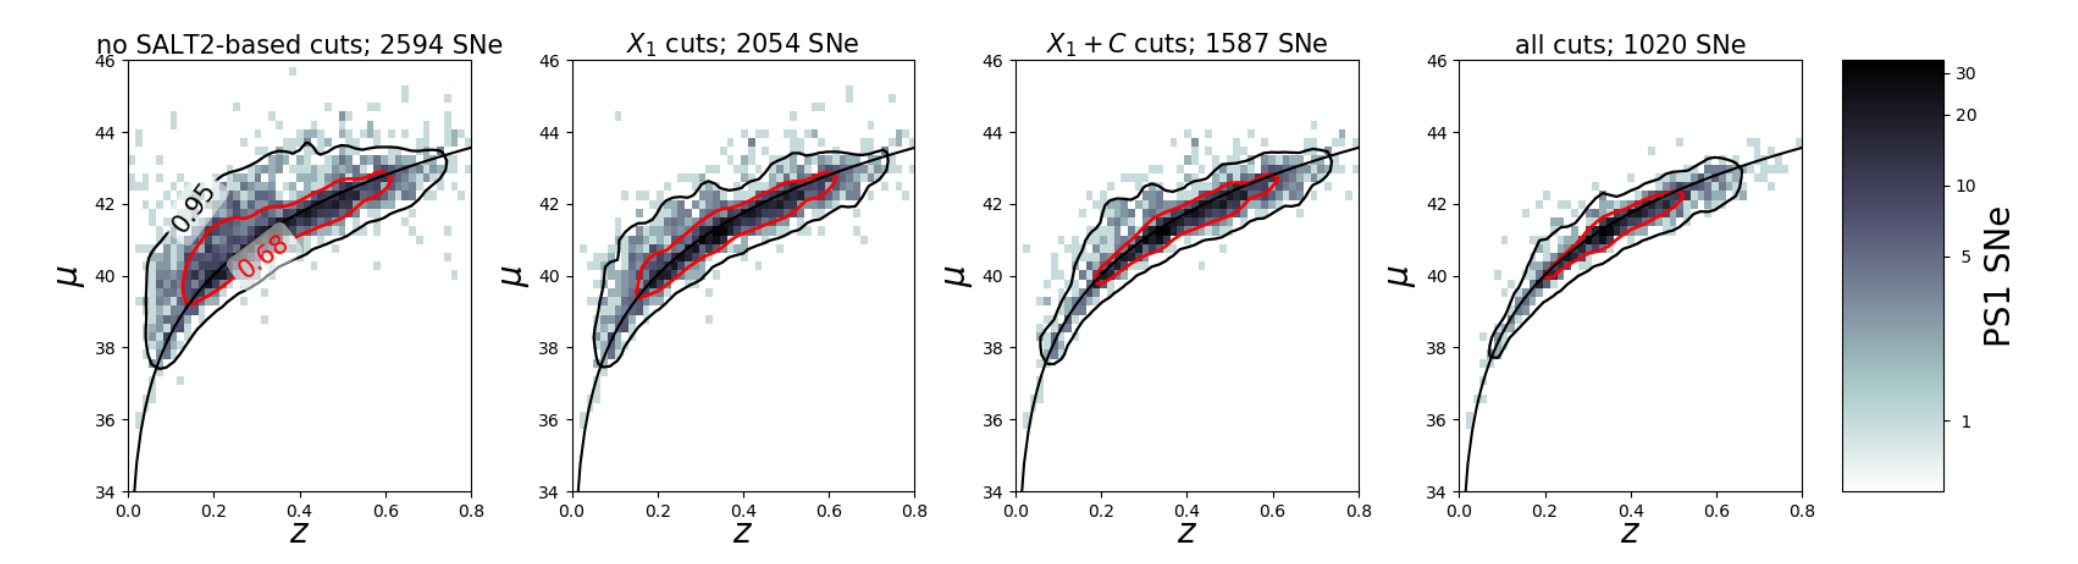
\includegraphics[width=1.0\textwidth]{fig/PanSTARRS.png}
\caption{{\bf Photometric and heterogeneous data:} data from the PanSTARRS survey show the spread in the distance modulus caused by objects with varying type probability.
Using cuts reduces this spread, but indeed removes some of the statistical power of the sample. 
Given faith in a classification algorithm and the resultant purity of the sample, these cuts can be justified, but including all the data weighted by the type probability provides a more robust treatment. 
Figure from \cite{Jones_2017}. \tkRH{[We need some attention grabbing plot rather than the graph to get people's attention!]  \textbf{()}}
\label{fig:intro}}
\end{center}
\end{figure*}
The future of supernova cosmology is photometric.
Ambitious survey telescopes like the Large Synoptic Survey Telescope (LSST) will yield more than two orders of magnitude mode `candidate' supernova detections, a combination of the more cosmologically useful Type Ia supernovae and interlopers of many different sorts of core-collapse events and other interesting objects.
Over the past decade, work has been intensifying to answer the question: \textit{'How does one perform cosmological analysis on a hetereogenous population of supernovae without certainty in the specific type of any object?'} \citet{kunz_bayesian_2007, kelly_flexible_2008, hlozek_photometric_2012, Lochner_2013, newling_2012}

The key concept in the above is a lack of certainty in the specific type.
While the sophistication of classification methods as applied to photometric data is improving greatly \tkRH{Note: Cite classification papers here}, most yield either a classification type `score' or some other proxy for probability of type (eg. from fitting the data to a suite of light curve templates from a specific type).
When selecting a final data set over which to test cosmological models, one then either makes a cut on probability of the Type Ia, or includes all the data in a Bayesian framework \citet{kunz_bayesian_2007, kelly_flexible_2008, hlozek_photometric_2012, Lochner_2013, newling_2012}.

Typing probability isn't, however, the only source of systematic error that must be considered for photometric surveys.
Indeed, photometric redshift uncertainties (and potential biases) are also important when fitting any models to a suite of data. 
The question above then becomes instead \textit{`How does one perform cosmological analysis on a hetereogenous population of supernovae without certainty in the specific type of any object nor the redshift of the object and its potential host?'}

The problem of inferring the cosmological parameters and redshift-dependent supernova type proportions from purely photometric data in the form of supernova lightcurves and host galaxy photometry is the next hurdle in any rigorous cosmological analysis, one that is beginning to be investigated by the community \citep{Roberts_2017}.
Our approach is to infer cosmological parameters and redshift-dependent supernova type proportions purely from photometric candidate (supernova) light curves and host galaxy photometry.
We describe the notation in Section~\ref{sec:method} and our method for simulating data in Section~\ref{sec:data}.

% \tkAM{Somewhere in the introduction, we should use this figure to emphasize the severity of the consequences of contamination.}
% \begin{figure*}
% \begin{center}
% 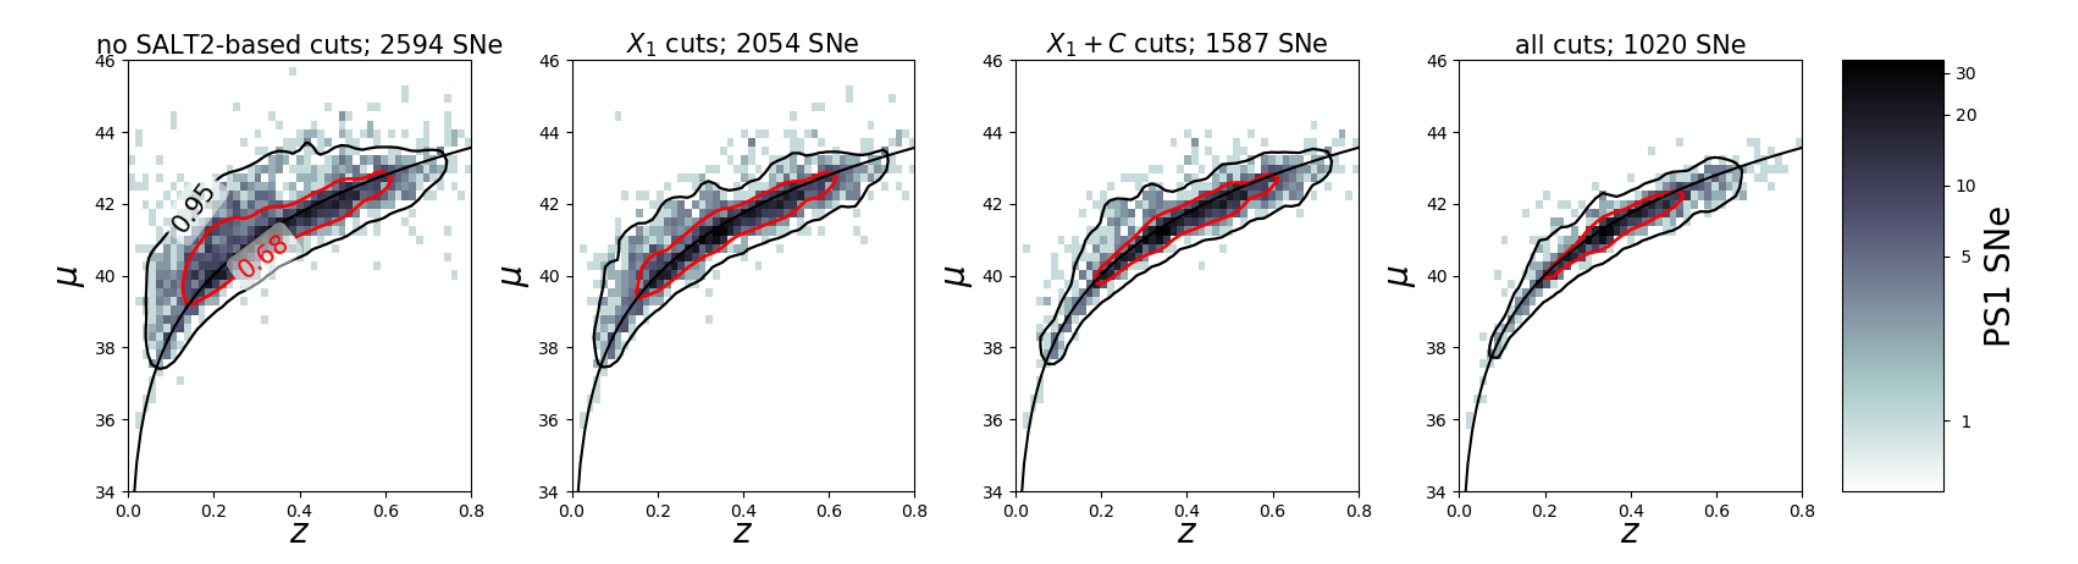
\includegraphics[width=1.0\textwidth]{fig/PanSTARRS.png}
% \caption{{\bf Photometric and heterogeneous data:} data from the Pan-STARRS survey show the spread in the distance modulus caused by objects with varying type probability. Using cuts reduces this spread, but indeed removes some of the statistical power of the sample. Given faith in a classification algorithm and the resultant purity of the sample, these cuts can be justified, but including all the data weighted by the type probability provides a more robust treatment. Figure from \cite{Jones_2017}. \tkRH{[We need some attention grabbing plot rather than the graph to get people's attention!]  \textbf{()}}
% \label{fig:intro}}
% \end{center}
% \end{figure*}

\section{Method}
\label{sec:method}

%This work demonstrates a principled approach to inferring cosmological parameters and redshift-dependent supernova type proportions from purely photometric lightcurves of supernovae and host galaxy photometry.  First, we outline the notation used throughout this paper.
%Let us consider a catalog of $N$ supernovae $n$, each with observed data comprised of a multi-band photometric lightcurve $\textul{\ell}_{n}$ and host galaxy photometry $\vec{f}_{n}$ comprised of fluxes, magnitudes, and/or colors.
%Every supernova has several intrinsic parameters that are not directly observable: a type $t_{n}$, a redshift $z_{n}$, and a distance modulus $\mu_{n}$.

%by assuming that the lightcurves and host galaxy photometry are random variables drawn from distributions that are functions of these unobservable parameters.

A photometric supernova catalog generally has observational data consisting of multi-band photometric lightcurves and host galaxy photometry comprised of fluxes, magnitudes, and/or colors. 
Each of the observed supernovae have intrinsic properties that are not directly observable, but we want to deduce: e.g. type, redshift, and distance modulus.  

Standard methods estimate the values of these unobservable parameters directly from the observed lightcurves and host galaxy redshift estimates.

However, these parameters are themselves determined by population-level \textit{hyper}parameters, including the SN type proportions (which are redshift dependent) and the cosmology (e.g. the Hubble parameter, $H_{0}$, and matter density, $\Omega_{0}$). 

The basis of the scippr model is both these two assumptions: the observed data of one SN is dependent on its true physical parameters and that the per-SN physical parameters are dependent on population-wide hyperparameters. 
This is implicit in all SN cosmology performed to date, but is rarely implemented as full hierarchical model. 
This has been done using lightcurve modeling, without host galaxy data, in the spectroscopic case in \cite{march/etal:2011}. 
The \SCIPPR method uses a full heirarchical model with only photometric data and incorporates host galaxy photometry.

\subsection{Model}
\label{sec:model}

The key idea with a Bayesian hierarchical model is that we are interested in estimating the hyperparameters directly, without first inferring the (in principle) unobservable parameters. 
In order to do this we take advantage of the causal relationships between the variables, as have outlined above, and outlined in a directed acyclic graph (DAG) in Fig.~\ref{fig:pgm}. 
The mathematical expressions for these causal relationships form a probabilistic graphical model (PGM).
The PGM shown in Figure~\ref{fig:pgm} includes two additional categories of complexity beyond the variables introduced above.

\tkAM{This is where we should clarify the statistical independence between SN and the selection function parameters.}  
%It is worth noting that we assume that the parameters associated with supernova $n$ and its host galaxy are statistically independent of the parameters associated with supernova $n'$ and its host galaxy.
%In addition to the parameters we have already introduced, there are two more in our model representing the selection functions in supernova lightcurves $\vec{\alpha}$ and host galaxy photometry $\vec{\beta}$.  \tkAM{Note: We will rename $\vec{\alpha}$ and $\vec{\beta}$.}



The motivation for this approach is the existence of photo-$z$ PDFs and the anticipation of PDFs over lightcurve fit parameters, like the colour or stretch in the cast of SALT-II.  
Photo-$z$ PDFs are posterior probability distributions; we observe the host galaxy photometry $\vec{f}_{n}$ and learn something about the host galaxy redshift $z_{n}$.  
The process by which we derive a relationship between the observed and unobserved parameters imprints its biases in the form of an interim prior that defines a global probability distribution over redshifts parametrized by $\vec{\theta}$.  
The selection function also biases the posterior probability in the form of an interim prior parametrized by $\vec{\beta}$.  
Thus photo-$z$ PDF is an interim posterior probability distribution $p(z_{n} | \vec{f}_{n}, \vec{\theta}, \vec{\beta})$.

We anticipate the production of lightcurve parameter PDFs, which will also be interim posterior probability distributions, but in a higher dimensional space.  
As in the case of photo-$z$ PDFs, the observed multi-band lightcurves $\{\vec{\ell}_{n}\}_{N}$ inform us about the latent parameters of supernova types $\{t_{n}\}_{N}$, redshifts $\{z_{n}\}_{N}$, and distance moduli $\{\mu_{n}\}_{N}$.  
The interim prior will be a probability distribution over $t$, $z$, and $\mu$ with known parameters comprising $\textul{\xi}$.  
We will also have a lightcurve selection function of parameters $\vec{\alpha}$ that is another distribution over this three-dimensional space.  
The overall interim posterior of the supernova lightcurve is then $p(t_{n}, z_{n}, \mu_{n} | \textul{\ell}_{n}, \textul{\xi}, \vec{\alpha})$.

\begin{figure}
\begin{center}
\includegraphics[width=0.55\textwidth]{fig/pgm.png}
\caption{This directed acyclic graph corresponds to a probabilistic graphical model for our hierarchical inference of the cosmological parameters and redshift-dependent type proportion parameters.  
In this graph, all random variables are shown in circles, with observed variables shown in shaded circles. 
The box indicates that there are $N$ copies of the relationships between boxed parameters, each statistically independent of all others.  
The hyperparameters we would like to infer are the cosmological parameters in $\vec{\Omega}$ and the redshift-dependent type proportion parameters comprising $\textul{\phi}$.  
Drawn from functions of these hyperparameters are the distance moduli $\{\mu_{n}\}_{N}$, redshifts $\{z_{n}\}_{N}$, and supernova types $\{t_{n}\}_{N}$.  
Here, we observe host galaxy colors $\{\vec{f}_{n}\}_{N}$ and multi-band supernova lightcurves $\{\textul{\ell}_{n}\}_{N}$, shown in shaded circles.  
The solid dots indicate known constants that factor into the model; $\vec{\alpha}$ represents the parameters defining a selection function in the space of observed lightcurves, and $\vec{\beta}$ includes the parameters defining a selection function in the space of host galaxy photometry.  
The arrows encode the relationships between variables, going from parameters defining probability distributions to variables drawn from those probability distributions.}
\label{fig:pgm}
\end{center}
\end{figure}

%We illustrate the flow of data through the \scippr process in Figure~\ref{fig:simflow}.
% \begin{figure*}
% \begin{center}
% 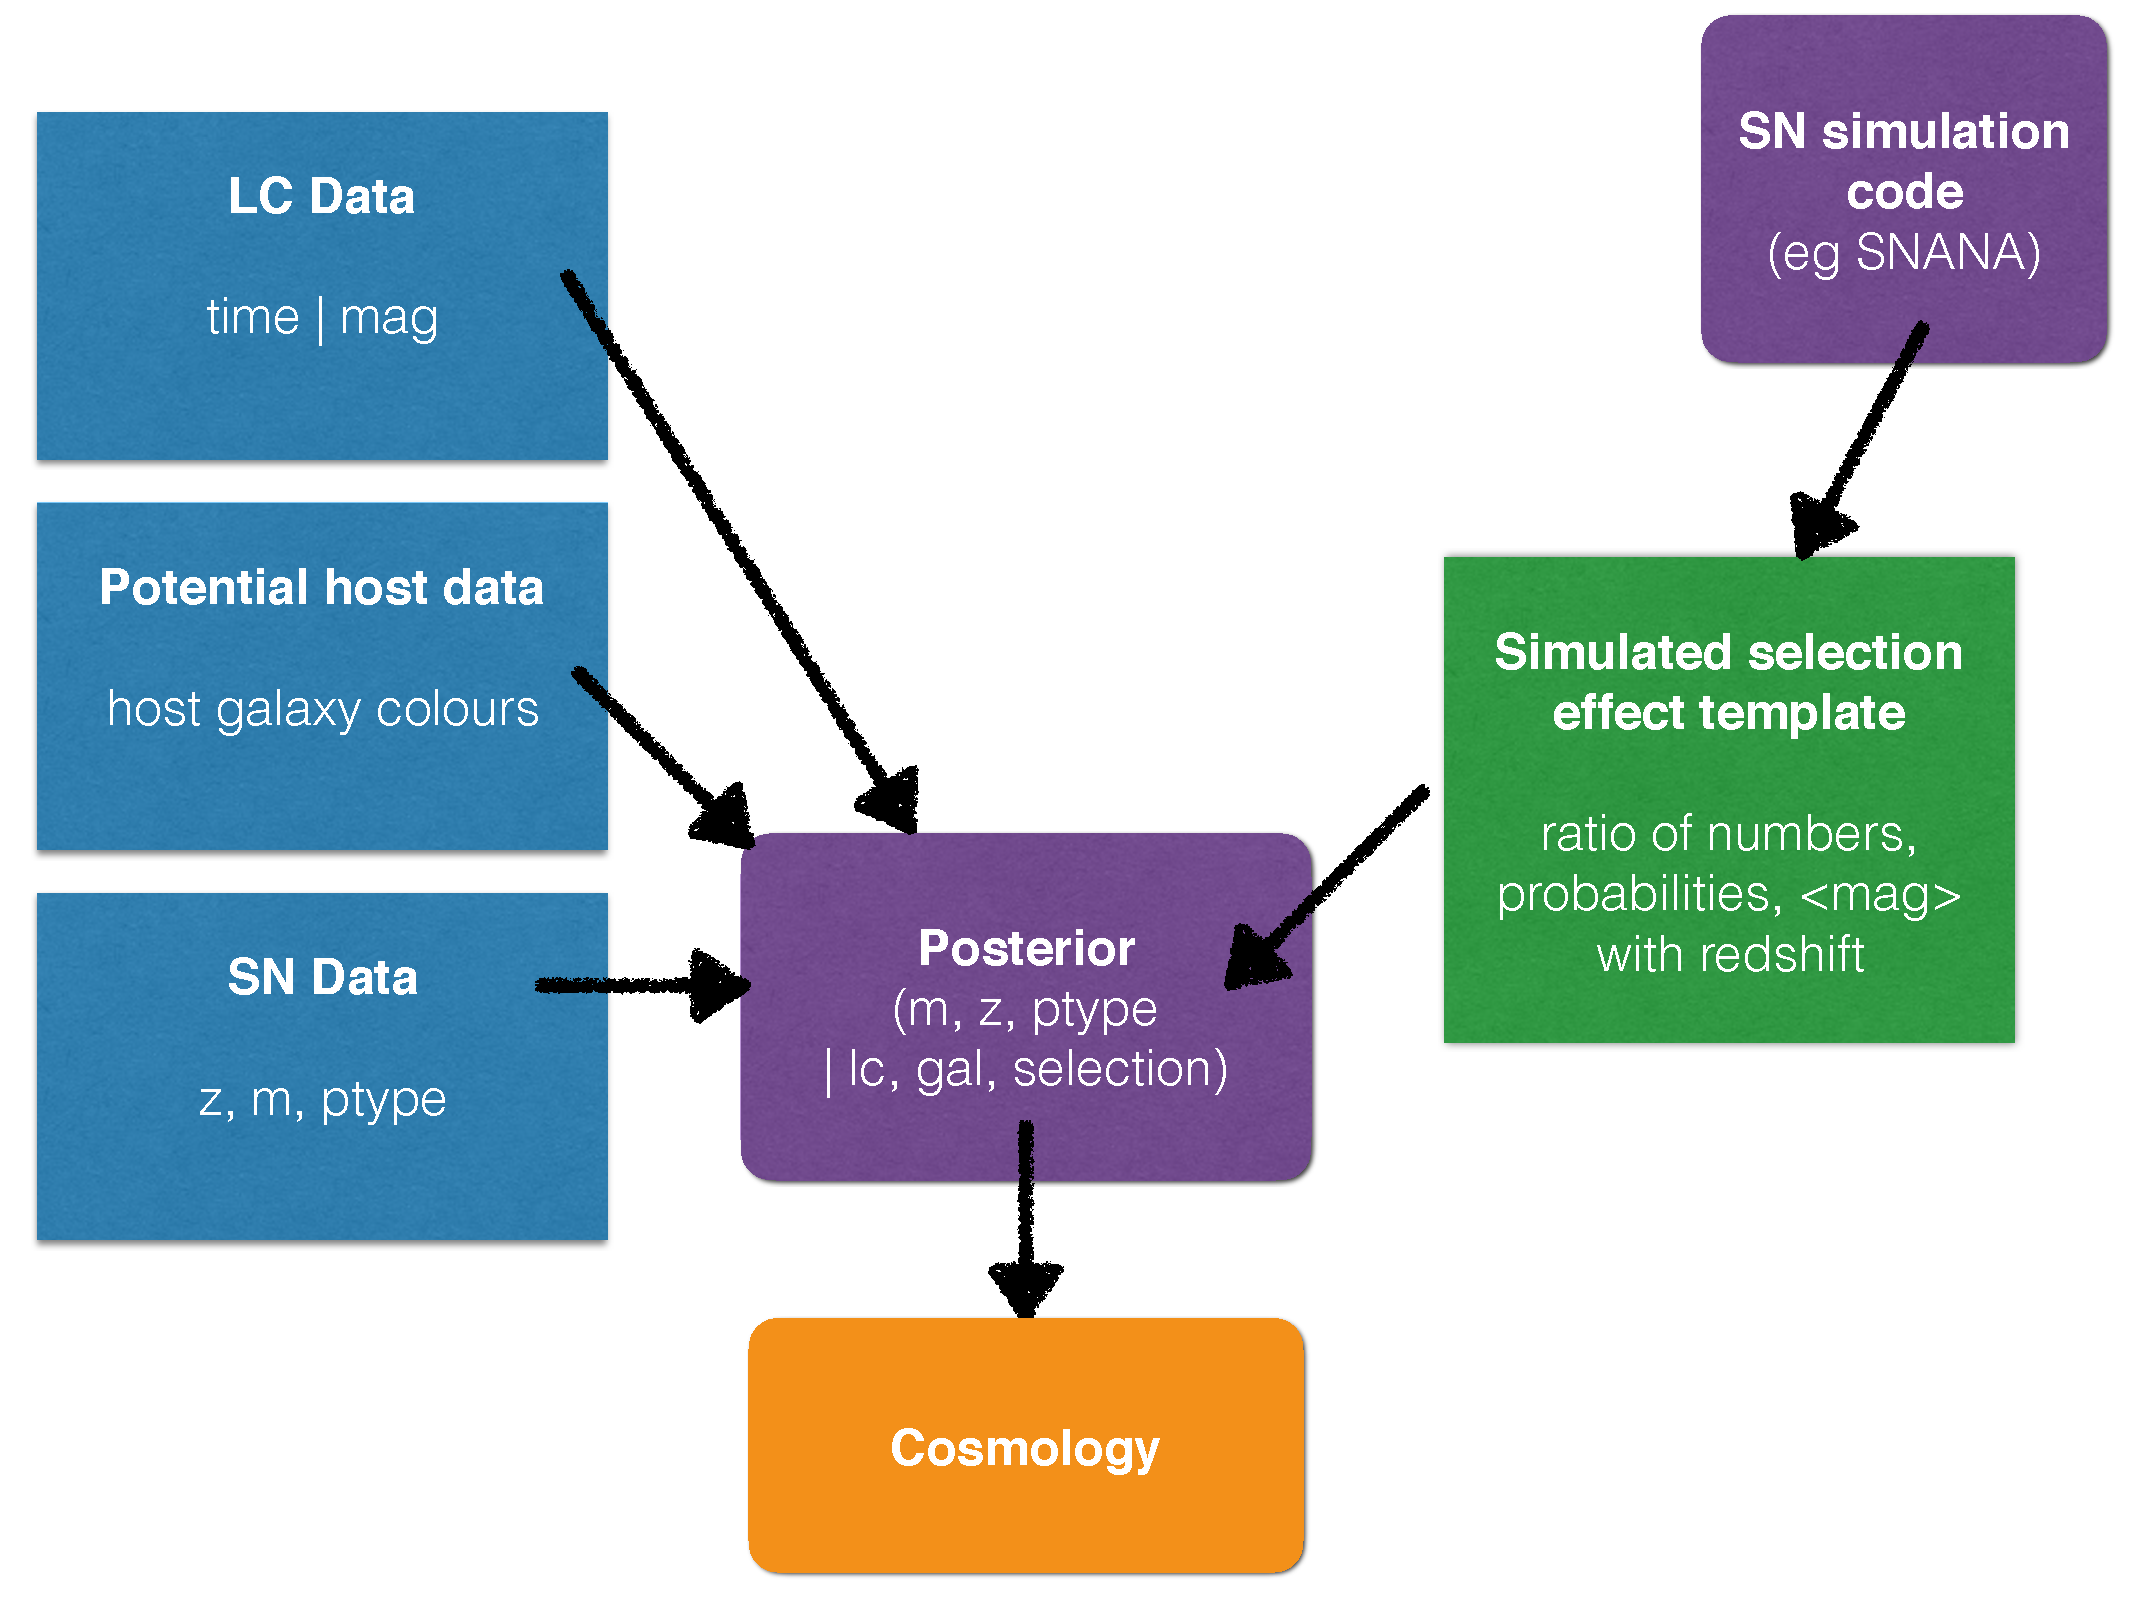
\includegraphics[width=1.0\textwidth]{fig/Schematic_Hlozek.pdf}\\
% \caption{{\bf The flow of the \scippr process:} by combining a prior-based selection function that is simulated for a given survey with the SN magnitudes, redshift and type and the potential host galaxy colours, the full posterior across both magnitude, type and galaxy properties is obtained 
% \label{fig:flow1}}
% \end{center}
% \end{figure*}

% \textbf{(@aimalz Discuss interim priors and selection functions in more detail here, or somewhere else?)}
% \tkAM{Maybe this belongs here, maybe elsewhere\dots}
When we conduct a photometric survey, not all supernovae in the universe will make it into our sample due to selection effects. 
These selection effects need to be included in any analysis to account for data that are excluded.

We proceed via the posterior distribution $p(\vec{\Omega}, \textul{\phi} | \{\textul{\ell}_{n}\}_{N}, \{\vec{f}_{n}\}_{N})$ of the physically important hyperparameters in $\vec{\Omega}$ (e.g. the cosmology you are trying to infer) and $\textul{\phi}$ (the parameters describing the relative proportions of different supernova populations as a function of redshift) given a catalog of $N$ interim posterior distributions of the type, redshift, distance modulus, $p(t_{n}, z_{n}, \mu_{n} | \textul{\ell}_{n}, \textul{\xi}, \vec{\alpha})$ specified by the parameters $\textul{\xi}$ describing the distributions of $t,z,\mu$ and the lightcurve selection function parameters $\vec{\alpha}$.
To infer the posterior distribution above we also need another $N$ interim posterior distributions $p(z_{n} | \vec{f}_{n}, \vec{\theta}, \vec{\beta})$, that specify the host-$z$ PDF.


The end goal is to derive an expression for the posterior distribution above over hyperparameters (which we want to obtain) in terms of the interim posteriors over latent parameters (which we know).

We begin by expanding this in terms of Bayes' Rule:
\begin{align}
\label{eq:bayes}
p(\vec{\Omega}, \textul{\phi} | \{\textul{\ell}_{n}\}_{N}, \{\vec{f}_{n}\}_{N}) &\propto p(\vec{\Omega}, \textul{\phi})\ p(\{\textul{\ell}_{n}\}_{N}, \{\vec{f}_{n}\}_{N} | \vec{\Omega}, \textul{\phi})
\end{align}

The \textit{posterior probability} of a certain cosmology and redshift-dependent type proportions given some set of observed supernova lightcurves and host galaxy photometry is proportional to the product the prior on the cosomological parameters; 
the redshift-dependent type proportions and the likelihood of the lightcurves and host galaxy photometry \textit{given} the cosmology and redshift-dependent type proportions.

A key assumption is the statistical independence of the supernova parameters and observations; 
each set of $(t_{n'}, z_{n'}, \mu_{n'}, \textul{\ell}_{n'}, \vec{f}_{n'})$ is independent from all other parameters in $\bigcup_{n}(t_{n\neq n'}, z_{n\neq n'}, \mu_{n\neq n'}, \textul{\ell}_{n\neq n'}, \vec{f}_{n\neq n'})$.
\begin{align}
\label{eq:independence}
p(\{\textul{\ell}_{n}\}_{N}, \{\vec{f}_{n}\}_{N} | \vec{\Omega}, \textul{\phi}) &= \prod_{n}^{N}p(\textul{\ell}_{n}, \vec{f}_{n} | \vec{\Omega}, \textul{\phi})
\end{align}

This assumption is necessary for us to easily combine the contributions of individual supernovae to the likelihood of the whole survey of supernovae. 
Here we are saying the the likelihood of the set of lightcurves and fluxes is simply the product of each of the individual likelihoods.

We give the full derivation of the posterior in Appendix~\ref{appendix:derivation}, including discussion of the assumptions we make and ways they might be relaxed. 
The final posterior on the cosmological parameters of interest and redshift-dependent type proportions is given as:

\begin{widetext}

\begin{eqnarray}
\label{eq:wrapupmain}
p(\vec{\Omega}, \textul{\phi} | \{\textul{\ell}_{n}, \vec{f}_{n}\}_{N}) &\propto& p(\vec{\Omega}, \textul{\phi}) \prod_{n}^{N}\ \iiint p(\mu_{n}, z_{n}, t_{n} | \textul{\ell}_{n}, \vec{f}_{n}, \vec{\theta}, \textul{\xi}, \vec{\alpha}, \vec{\beta}) \times \frac{p(\mu_{n}, z_{n}, t_{n} | \vec{\Omega}, \textul{\phi})}{p(\mu_{n}, z_{n}, t_{n} | \vec{\theta}, \textul{\xi}, \vec{\alpha}, \vec{\beta})}\ d\mu_{n}\ dz_{n}\ dt_{n},
\end{eqnarray}
\end{widetext}

We implement the model of Sec. \ref{sec:model} in the form of the Supernova Cosmology Inference with Probabilistic Photometric Redshifts code \scippr, which is a \texttt{Python} code freely available to the community. 


\section{Mock Data}
\label{sec:data}
The biggest difference between \SCIPPR and the standard approach is the fact that the traditional Hubble diagram of $z, \mu(z)$ is absent, given that the input data are light curve points and host galaxy fluxes/colours, as described above, interacting with light curve/photo-$z$ codes to produce \textit{joint interim posteriors} over redshift and distance modulus.

For the supernova fitting/classification codes these would run over the combinations of supernova type $t$ and distance modulus $\mu$ and redshift $z$ based on supernova light curves $l_c$ which are provided by supernova light curve fitters, $p(t_{i}, z_{i}, \mu_{i} | \textul{\ell}_{i})\ \equiv\ p(t_{i}, z_{i}, \mu_{i} | t_{i},' z_{i}', \mu_{i}'),$ while for the host galaxy photo-$z$ codes these would run over redshift $z$ given the host galaxy photometry $f$, $p(z_{i} | \vec{f}_{i})$ as shown in the two boxes side-by-side in Figure~\ref{fig:simflow}.  

Developing codes that produce these interim priors is an active area of research in the community, however such codes are not currently publicly available to produce the joint distributions. 
% As was mentioned in Sec. \ref{sec:model}, it is nontrivial to confirm the accuracy of any probabilistic data analysis method, and so developing such a code pipeline for producing the joint distributions is left to future work.

Here we directly simulate these two interim posteriors and obtain the joint distribution, $p(\{\mu_{i}, z_{i}, t_{i}\}_{N} | \{\textul{\ell}_{i}, \vec{f}_{i}\}_{N}, \textul{\Phi}^{*}, \vec{\varphi}^{*}, \vec{\alpha}, \vec{\beta})$, which is shown as the lower box at the bottom of Figure~\ref{fig:simflow}.

In this section, we outline the forward model we use to simulate the interim posteriors as our `data'.

\begin{figure*}
\vspace{0.5cm}
\begin{center}
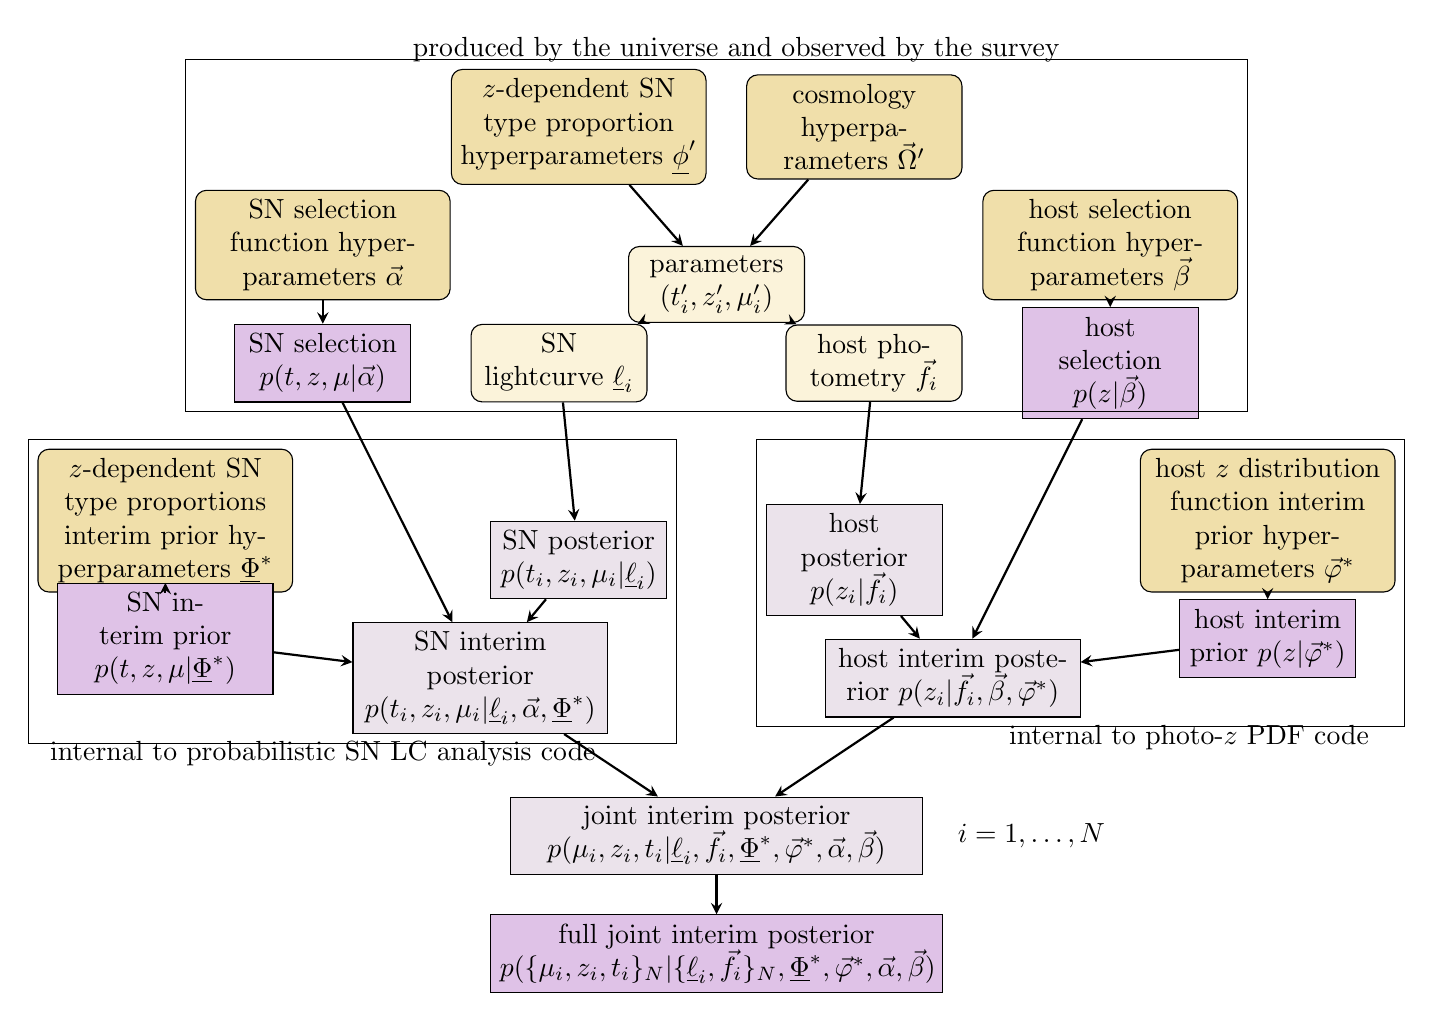
\begin{tikzpicture}[node distance=1cm]

\node (joint) [probperSN, text width=5cm] {joint interim posterior $p(\mu_{i}, z_{i}, t_{i} | \textul{\ell}_{i}, \vec{f}_{i}, \textul{\Phi}^{*}, \vec{\varphi}^{*}, \vec{\alpha}, \vec{\beta})$};

\node (fulljoint) [globalprob, below of=joint, text width=5.5cm, yshift=-0.5cm] {full joint interim posterior $p(\{\mu_{i}, z_{i}, t_{i}\}_{N} | \{\textul{\ell}_{i}, \vec{f}_{i}\}_{N}, \textul{\Phi}^{*}, \vec{\varphi}^{*}, \vec{\alpha}, \vec{\beta})$};

\node (fullhost) [probperSN, above of=joint, xshift=3.0cm, yshift=1.0cm, text width=3.0cm] {host interim posterior $p(z_{i} | \vec{f}_{i}, \vec{\beta}, \vec{\varphi}^{*})$};
\node (fullSN) [probperSN, above of=joint, xshift=-3.0cm, yshift=1.0cm, text width=3.0cm] {SN interim posterior $p(t_{i}, z_{i}, \mu_{i} | \textul{\ell}_{i}, \vec{\alpha}, \textul{\Phi}^{*})$};

\node (hostpost) [probperSN, above of=fullhost, xshift=-1.25cm, yshift=0.5cm, text width=2.0cm] {host posterior $p(z_{i} | \vec{f}_{i})$};
\node (SNpost) [probperSN, above of=fullSN, xshift=1.25cm, yshift=0.5cm, text width=2.0cm] {SN posterior $p(t_{i}, z_{i}, \mu_{i} | \textul{\ell}_{i})$};

\node (trueparams) [valsperSN, above of=joint, yshift=6.0cm, text width=2.0cm] {parameters $(t'_{i}, z'_{i}, \mu'_{i})$};

\node (LCdata) [valsperSN, below of=trueparams, xshift=-2.0cm, text width=2.0cm] {SN lightcurve $\textul{\ell}_{i}$};
\node (hostdata) [valsperSN, below of=trueparams, xshift=2.0cm, text width=2.0cm] {host photometry $\vec{f}_{i}$};

\node (truecosmo) [globalvals, above of=trueparams, xshift=1.75cm, yshift=1.0cm, text width=2.5cm] {cosmology hyperparameters $\vec{\Omega}'$};
\node (trueprops) [globalvals, above of=trueparams, xshift=-1.75cm, yshift=1.0cm, text width=3.0cm] {$z$-dependent SN type proportion hyperparameters $\textul{\phi}'$};

\node (SNintprparam) [globalvals, left of=fullSN, xshift=-3.0cm, yshift=2.0cm, text width=3.0cm] {$z$-dependent SN type proportions interim prior hyperparameters $\textul{\Phi}^{*}$};
\node (hostintprparam) [globalvals, right of=fullhost, xshift=3.0cm, yshift=2.0cm, text width=3.0cm] {host $z$ distribution function interim prior hyperparameters $\vec{\varphi}^{*}$};

\node (hostintpr) [globalprob, below of=hostintprparam, yshift=-0.5cm, text width=2.0cm] {host interim prior $p(z | \vec{\varphi}^{*})$};
\node (SNintpr) [globalprob, below of=SNintprparam, yshift=-0.5cm, text width=2.5cm] {SN interim prior $p(t, z, \mu | \textul{\Phi}^{*})$};

\node (SNselfunparam) [globalvals, left of=trueparams, xshift=-4.0cm, yshift=0.5cm, text width=3.0cm] {SN selection function hyperparameters $\vec{\alpha}$};
\node (hostselfunparam) [globalvals, right of=trueparams, xshift=4.0cm, yshift=0.5cm, text width=3.0cm] {host selection function hyperparameters $\vec{\beta}$};

\node (hostselfun) [globalprob, below of=hostselfunparam, yshift=-0.5cm, text width=2.0cm] {host selection $p(z | \vec{\beta})$};
\node (SNselfun) [globalprob, below of=SNselfunparam, yshift=-0.5cm, text width=2.0cm] {SN selection $p(t, z, \mu | \vec{\alpha})$};

% \node (survey) [draw=black,  fit=(fullSN.west)(trueparams.north)(joint.south)(fullhost.east)] 
% {};
\node [xshift=4.0cm, yshift=0.5cm] at (joint.south) {$i=1,\dots,N$};

\node (obs) [draw=black,  fit=(SNselfunparam.west)(trueprops.north)(hostdata.south)(hostselfunparam.east)] 
{};
\node [xshift=2.0cm,yshift=0.25cm] at (trueprops.north) {produced by the universe and observed by the survey};

\node (SNanalysis) [draw=black,  fit=(SNintprparam.west)(SNintprparam.north)(fullSN.south)(SNpost.east)]
{};
\node [xshift=-2.0cm,yshift=-0.25cm] at (fullSN.south) {internal to probabilistic SN LC analysis code};

\node (hostanalysis) [draw=black,  fit=(hostintprparam.east)(hostintprparam.north)(fullhost.south)(hostpost.west)]
{};
\node [xshift=3.0cm,yshift=-0.25cm] at (fullhost.south) {internal to photo-$z$ PDF code};

\draw [arrow] (fullhost) -- (joint);
\draw [arrow] (fullSN) -- (joint);
\draw [arrow] (hostselfunparam) -- (hostselfun);
\draw [arrow] (hostselfun) -- (fullhost);
\draw [arrow] (hostintprparam) -- (hostintpr);
\draw [arrow] (hostintpr) -- (fullhost);
\draw [arrow] (hostpost) -- (fullhost);
\draw [arrow] (SNselfunparam) -- (SNselfun);
\draw [arrow] (SNselfun) -- (fullSN);
\draw [arrow] (SNintprparam) -- (SNintpr);
\draw [arrow] (SNintpr) -- (fullSN);
\draw [arrow] (SNpost) -- (fullSN);
\draw [arrow] (truecosmo) -- (trueparams);
\draw [arrow] (trueprops) -- (trueparams);
\draw [arrow] (trueparams) -- (hostdata);
\draw [arrow] (trueparams) -- (LCdata);
\draw [arrow] (hostdata) -- (hostpost);
\draw [arrow] (LCdata) -- (SNpost);
\draw [arrow] (joint) -- (fulljoint);

\end{tikzpicture}
\caption{An illustration of the mock data generation procedure.  
Rounded, yellow boxes represent parameter values, whereas squared, purple boxes represent probability distributions.  
Lighter colors represent quantities defined for each supernova-host galaxy pair in a survey, whereas darker colors represent quantities shared across all observed objects.}
\label{fig:simflow}
\end{center}
\end{figure*}

 \subsection{Distances, redshifts and types:the true hyperparameters and parameters}
\label{sec:true_hypers}

We begin by choosing parametrizations for the true underlying parameters of interest (the cosmology), and the hyperparameters to generate the \textit{distributions} from which the supernova type $t$, redshift $z$, and distance modulus $\mu$ are drawn.

% 
\subsubsection{The relative proportions of supernova types}
\label{sec:sntypes}

\begin{table*}
    \begin{tabular}{| l | c | c | c |}
    \hline
    & Ia & Ibc & II \\ \hline
	\parbox{4cm}{\flushleft true cosmology hyperparameters \\ } & \multicolumn{3}{|c|}{\cite{Planck2016}} \\ \hline
	
	\parbox{4cm}{\flushleft supernova type ratios as a function of redshift \\ } & \multicolumn{3}{|c|}{$p(t,z | \phi)$} \\ \hline
	
	\parbox{4cm}{\flushleft number of SNe per volume per redshift \\ } & \parbox{4cm}{\flushleft $\Psi$: delay time distribution} &  \parbox{4cm}{?} & \parbox{4cm}{\flushleft $K_{II}$: fraction of stars that explode as SNII \citep{Salpeter1955}} \\ 
	{} & \parbox{4cm}{\flushleft $SFH$: cosmic star formation history} &  \parbox{4cm}{?} & \parbox{4cm}{\flushleft $SFR$: Star formation rate (\citealt{Cole2001}, \citealt{Horiuchi2011}, \citealt{Madau2014})} \\
	{} & \parbox{4cm}{\flushleft $R_{Ia}(t) = \int_{0}^{t} S(t - \tau)\Psi(\tau)d\tau$ \cite{Graur_2013}} &  \parbox{4cm}{?} & \parbox{4cm}{\flushleft $R_{II}$ = $K_{II}$ x $SFR$} \\ \hline
	
	\parbox{4cm}{\flushleft spectral models as a function of time \\ } & SN Ia 1994D &  ? & \parbox{4cm}{\flushleft CSP-like SNe II simulated using MCMC} \\ \hline
	
	\parbox{4cm}{\flushleft K-corrections between bands} & \cite{Hsiao2007} &  ? & \cite{Dessart2013} \\ \hline
	
	\parbox{4cm}{\flushleft LSST filter throughputs \\ } & \multicolumn{3}{|c|}{\parbox[c]{8cm}{\flushleft SysEng-approved LSST throughput curves \\ github.com/lsst/throughputs/tree/master/baseline \\ }} \\ \hline
	
	\parbox{4cm}{\flushleft LSST single epoch limiting magnitudes \\ } & \multicolumn{3}{|c|}{\parbox[c]{8cm}{\flushleft \cite{LSSTScienceBook} \\ $u$=23.60 $g$=24.83 $r$=24.38 $i$=23.92 $z$=23.35 \\ }} \\ \hline
	
	\parbox{4cm}{\flushleft Classified types of detected light curves} & ? & ? & ? \\ \lasthline
    \end{tabular}
\caption{Supernova rates calculation process.}
\label{table:name}
\end{table*}

\vspace{1cm}
To simulate different supernova types as a function of redshift, we parameterize the proportions of different supernova types relative to each other. 
These proportions will depend on properties such as the cosmological star formation history and the absolute magnitude of the objects, and as such will be redshift-dependent.

We model this redshift-dependent proportion $p(t, z | \textul{\phi})$, as a two-dimensional piecewise constant function over $N_t$ types and $N_z$ redshift bins, making $\textul{\phi}$ a $N_t\times N_z$ array with values $\phi_{i}$ equal to the \textit{probability of a supernova being of type $t$ with a redshift $z$ in a given bin}.  
A normalization condition is enforced such that summing over the discrete variable of supernova type and integrating over all redshift bins yields a value of unity.

To demonstrate the evolutionary relationship between \BEAMS and \SCIPPR, we consider $N_t=3$, with $\tau\in\{Ia, Ibc, II\}$. 
Under this parametrization, we use realistic values for the elements of $\textul{\phi}'$ derived by convolving the delay time distribution (DTD) and the star formation history.  
We discuss the specific forumltion of the rates in the Appedix, Secs. \ref{sec:TypeIaRate}, \ref{sec:TypeIbcRate}, and \ref{sec:TypeIIRate}. 

As an overview, we set the relative rates of SN Ia and Core Collapse to be 25\% and 75\%, respectively, at z = 0.  \textbf{(@tinapeters How were these numbers modified for three SN populations?)} 
\textbf{(RH: this needs adjusting for the true simulation)}

We use the DTD for SN Ia from \cite{graur/etal:2013} and the DTD for SN II from \cite{zapartas/etal:2017}, and the Cosmic Star Formation Rate from \cite{behroozi/etal:2013}. 
The redshift-dependent supernova type proportions derived in this way are shown in Fig. \ref{fig:relative_supernova_rates}, where $N=10^{4}$ pairs of $(t'_{n}, z'_{n})$ are drawn from this distribution.  \textbf{(@tinapeters What is the native format of these curves, i.e. a continuous function evaluated on a grid or something else?  I wrote about a piecewise constant function, but it can and should be whatever's consistent with the actual functions you calculated.)}  

\begin{figure}
	\begin{center}
		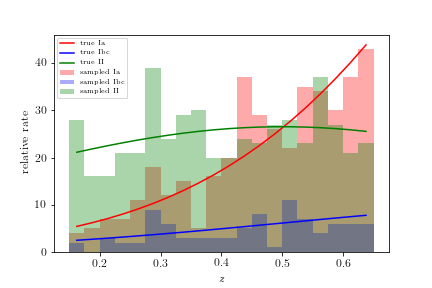
\includegraphics[width=0.5\textwidth]{fig/obs_rates.png}
		\caption{The simulated types and redshifts of 1000 supernovae.}
		\label{fig:obs_rates}
	\end{center}
\end{figure}


\subsubsection{Cosmological parameters}
\label{sec:cosmohypers}

For the parametrization of the cosmological parameters, we assume a $\Lambda$CDM cosmology so $\vec{\Omega}$ is comprised of $\vec{\Omega} = \{H_{0}, \Omega_{m}, w\}$, where $H_0$ is the Hubble constant in units of $km/s/\mathrm{Mpc}$, $\Omega_m$ is the matter density and $w$ is the dark energy equation-of-state parameter. We assume flatness and so set the dark energy density to be $\Omega_\Lambda = 1-\Omega_m$.  
We choose the cosmological hyperparameters comprising $\vec{\Omega}'$ to be the maximum likelihood point estimates observed by Planck: $H_{0}=67.9\ km/s/\mathrm{Mpc}$ and $\Omega_{m}=0.307$.  \textbf{(@aimalz fix these constants here and in code)}  

These are used to generate the true distance modulus function at a given $z_{n}$:

\begin{widetext}
\begin{align}
\label{eq:distmod}
\mu(z) &= 5\log\left[(1+z)\frac{1}{10\ pc}\int_{0}^{z}\frac{dz'}{\sqrt{\Omega_{M}(1+z)^{3}+\Omega_{k}(1+z)^{2}+\Omega_{\Lambda}}}\right].
\end{align}
\end{widetext}

This means that once the pair $(t'_{n}, z'_{n})$ is drawn from the type interim posterior $p(t, z | \textul{\phi}')$ defined above, the posterior on the distance modulus \textit{given} the cosmology and redshift, $p(\mu_{n} | \vec{\Omega}', z'),$ is a $\delta$-function centered at $\mu'_{n}$ following Eq.~\ref{eq:distmod}.  

We have now set the true values of the hyperparameters (describing the cosmology and the type proportions) and the parameters describing the distances, redshifts and types.

\subsubsection{From parameters $t'_i,\mu'_i, z'_i$ posteriors}
\label{sec:drawmock}

With the hyperparameters describing cosmology and type proportions set in Section~\ref{sec:true_hypers}, the resulting \textit{true parameters} of  $\{(t_{i}', z_{i}', \mu_{i}')\}_{N}$ can be obtained.

%in Figure \ref{fig:obs_rates}

The intermediate estimated parameters are the supernova types $\{t_{n}\}_{N}$, redshifts $\{z_{n}\}_{N}$, and distance moduli $\{\mu_{n}\}_{N}$, which are derived from the observations of light curve points and fluxes:$p(\mu_{n}, z_{n}, t_{n} | \textul{\ell}_{n}, \vec{f}_{n})$. 

These estimated parameters $t_i,z_i,\mu_i$ enter into the SN interim join posteriors (see the light purple boxes in Figure~\ref{fig:simflow}).

%These can be thought of the types, redshifts and distance moduli that are estimated from observations.

%\textbf{repeated text}
%For the supernova type and redshift dimensions, we adopt the same parametrization used for $\textul{\phi}$.  There are $T$ supernova types and $Z$ redshift bins, indexed by $\tau$ and $\zeta$ respectively, and $D$ bins in distance modulus indexed by $\nu$.  $\textul{\phi}$ describes 

%Because the relative proportions of supernova types are parametrized by $\textul{\phi}'$ such that $p(z\in\zeta, t=\tau | \textul{\phi}') = \phi_{\zeta\tau}$, it is easy to draw pairs of true types and redshifts $(t_{n}', z_{n}')$ from $\textul{\phi}'$.  We treat the elements of $\textul{\phi}'$ as a discrete distribution, noting that the redshift-dependent supernova type proportions are normalized such that $\sum_{\tau}\int_{\zeta}\textul{\phi}=1$. 
%\textbf{Renee to make this clearer - we repeat ourselves! latent vs true is not clear here}

%As such, sampling the function defined by $\textul{\phi}'$ is equivalent to sampling true types and redshift bins. In our simulation then, we sample directly in type and redshift: oncce the redshift bins have been chosen, we may choose a true redshift for each supernova from a uniform distribution defined between the bin endpoints.  This procedure gives us pairs of true types and redshifts $(t_{n}', z_{n}')$.

%Finally, we calculate the true $\mu_{n}'$ according to  from $z_{n}'$ and $\vec{\theta}'$.  Rather than writing the form of the distance modulus as a function of redshift and cosmological parameters throughout the paper, we will instead use the shorthand $\mu = f_{\vec{\theta}}(z)$ here.  This results in a true catalog of length $N$ consisting of trios $(t_{n}', z_{n}', \mu_{n}')$ of the latent variables.

\subsection{Supernova lightcurve-based PDFs}
\label{sec:snlcpdf}

Each supernova in the sample must have a three-dimensional probability distribution, which will be an interim posterior, over the type, redshift, and distance modulus, combined as

\begin{widetext}
\begin{align}
    \label{eq:fullsnlcpdf}
    p(t, z, \mu | \textul{\ell}_{i}, \vec{\alpha}, \textul{\Phi}^{*}) = p(t, z, \mu | t_{i}', z_{i}', \mu_{i}', \vec{\alpha}, \textul{\Phi}^{*}) &= p(t, z, \mu | t_{i}', z_{i}', \mu_{i}')\ p(t, z, \mu | \textul{\Phi}^{*})] p(t, z, \mu | \vec{\alpha}),
\end{align}
 or in words,
\begin{eqnarray}
    \label{eq:fullsnlcpdfwords}
    [\textrm{supernova post-selection interim posterior}]_{i} &=& [\textrm{lightcurve posterior}]_{i}\ \boldsymbol{\cdot}\ \textrm{type-$z$-$\mu$ interim prior}\ \boldsymbol{\cdot}\nonumber \\ &&\textrm{supernova selection function}.
\end{eqnarray}

\end{widetext}

Sections \ref{sec:snlcposterior, sec:snlcinterim, sec:snlcselection} cover the production of the lightcurve posteriors, the type-redshift-distance modulus interim prior, and supernova selection function respectively.

\subsubsection{Supernova lightcurve data model}
\label{sec:snlcposterior}

\tkAM{We might want to revise this section to use the conditional probability table introduced in the PLAsTiCC metrics paper.}

We present our model for emulating three-dimensional posteriors $p(t, z, \mu | \textul{\ell}_{i})\equiv p(t, z, \mu | t_{i}', z_{i}', \mu_{i}')$.  
In current analyses, supernovae are classified before the lightcurve is fit, so we first emulate $p(t | t_{i}')$ using a typical confusion matrix of an unspecified classifier.  
The confusion matrix, illustrated in Table \ref{tab:confusionmatrix} has elements of $p(t', t)$, where $t'$ is the true type of a supernova and $t$ is the classified type.  
We note that the confusion matrix satisfies a normalization condition $\sum_{t'}\sum{t}p(t', t)=1$.  
By invoking Bayes' Rule, we can derive the desired classification probabilities $p(t | t')=p(t', t)/p(t')$.  
We know $p(t')$ for our mock data because we set $\textul{\phi}'$, and the confusion matrix provides $p(t', t)=p(t', t)$.  
In reality, not all supernovae of a single true type will have the same type posterior $p(t | \textul{\ell}_{i})$, but we make use of this simplification for now because we do not know enough about the output of a fully probabilistic lightcurve classifier to make a more realistic model.  
For these purposes we use the confusion matrix of\dots \textbf{(Choose a particular classifier's confusion matrix!)}

% \vspace{1in}
% \begin{figure}
% \renewcommand\arraystretch{1.5}
% \setlength\tabcolsep{0pt}
\begin{widetext}

\begin{tabular}{l @{\hspace{0.7em}}r @{\hspace{0.7em}}c @{\hspace{0.4em}}c @{\hspace{0.4em}}c @{\hspace{0.7em}}l}
    \multirow{17}{*}{\rotatebox{90}{\parbox{3.0cm}{\bfseries\centering Simulation Input}}} & & \multicolumn{3}{c}{\bfseries Classification Output} &  \\
	 & & $t = \RN{1}a$ & $t = \RN{1}bc$ & $t = \RN{2}$ & \bfseries total \\
	& \em{t' = \RN{1}a} & \MyBox{$p(t' = \RN{1}a, t = \RN{1}a)$}{ \ } & \MyBox{$p(t' = \RN{1}a, t = \RN{1}bc)$}{ \ } & \MyBox{$p(t' = \RN{1}a, t = \RN{2})$}{ \ } & Simulated \RN{1}a Rate \\[2.4em]
	& \em{t' = \RN{1}bc} & \MyBox{$p(t' = \RN{1}bc, t = \RN{1}a)$}{ \ } & \MyBox{$p(t' = \RN{1}bc, t = \RN{1}bc)$}{ \ } & \MyBox{$p(t' = \RN{1}bc, t = \RN{2})$}{ \ } & Simulated Ibc Rate\\[2.4em]
	& \em{t' = \RN{2}} & \MyBox{$p(t' = \RN{2}, t = \RN{1}a)$}{ \ } & \MyBox{$p(t' = \RN{2}, t = \RN{1}bc)$}{ \ } & \MyBox{$p(t' = \RN{2}, t = \RN{2})$}{ \ } & Simulated II Rate \\
    & {\bfseries total} & Classified \RN{1}a rate & Classified Ibc rate & Classified II rate & \\
    \label{tab:confusionmatrix}
\end{tabular}
%\caption{}
% \label{fig:confusion}
% \end{figure}

\end{widetext}

Next, we emulate $p(z, \mu | t, t'_{i}, z'_{i}, \mu'_{i})$, the redshift and distance modulus probabilities fit to a lightcurve given its classification, a three-dimensional object defined over dimensions of supernova type, redshift, and distance modulus.  
We know $p(z, \mu | t=\mathrm{Ia}, t'_{i}=\mathrm{Ia}, z'_{i}, \mu'_{i})$ from the output of successful lightcurve fits.  
Here, we use a bivariate Gaussian distribution $\mathcal{N}([z_{i}''^{\ell}, \mu_{i}''^{\ell}], \Sigma_{Ia})$ with a covariance $\Sigma_{Ia}$ shared by the entire dataset and a mean of $[z_{i}''^{\ell}, \mu_{i}''^{\ell}]$ drawn from a bivariate Gaussian distribution $\mathcal{N}([z'_{i}, \mu'_{i}], \Sigma_{Ia})$ of the same covariance with a mean of $[z'_{i}, \mu'_{i}]$, the true redshift and distance modulus.  

Since only type Ia supernovae are standardizable candles, we note that $p(z, \mu | t\neq\mathrm{Ia}, t'_{i}, z'_{i}, \mu'_{i})$ ought to be flat in the $\mu$ dimension.  
We also have some idea of what $p(z, \mu | t=\mathrm{Ia}, t'_{i}\neq\mathrm{Ia}, z'_{i}, \mu'_{i})$ should look like from contaminated Hubble diagrams.  \textbf{(Let's find one such plot!)}  
For $t'_{i}=\mathrm{Ibc}$, we use a bivariate Gaussian distribution $\mathcal{N}([z_{i}''^{\ell}, \mu_{i}''^{\ell}], \Sigma_{Ibc})$ with a covariance $\Sigma_{Ibc}$ shared by the entire dataset and a mean of $[z_{i}''^{\ell}, \mu_{i}''^{\ell}]$ drawn from a bivariate Gaussian distribution $\mathcal{N}([z'_{i}, \mu'_{i}-\mu_{Ibc}], \Sigma_{Ibc})$ of the same covariance with a mean of $[z'_{i}, \mu'_{i}-\mu_{Ibc}]$, the true redshift and a distance modulus downshifted from the true distance modulus by a constant $\mu_{Ibc}$ shared across the entire dataset.  
For $t'_{i}=\mathrm{II}$, we use a bivariate Gaussian distribution $\mathcal{N}([z_{i}''^{\ell}, \mu_{i}''^{\ell}], \Sigma_{II})$ with a covariance $\Sigma_{II}$ shared by the entire dataset and a mean of $[z_{i}''^{\ell}, \mu_{i}''^{\ell}]$ drawn from a bivariate Gaussian distribution $\mathcal{N}([z'_{i}, \mu_{II}], \Sigma_{II})$ of the same covariance with a mean of $[z'_{i}, \mu_{II}]$, the true redshift and a constant distance modulus $\mu_{II}$  shared across the entire dataset.  \textbf{(We're going to redo this with constants derived from an LSST-like analysis: make LSST-like lightcurves with SNANA, fit as Ia with PSNID, make better sheetcake model based on Hubble diagrams in each cell of confusion matrix.  We will make a plot of $p(t, z, \mu | t')$ for all $t$.)} \tkAM{We really need to use macros here to make it manageable to edit.}

Finally, we combine then terms as $p(t, z, \mu | \textul{\ell}_{i})\equiv p(t, z, \mu | t_{i}', z_{i}', \mu_{i}')=p(t | t'_{i})p(z, \mu | t'_{i}, z'_{i}, \mu'_{i})$.

\begin{figure}
	\begin{center}
		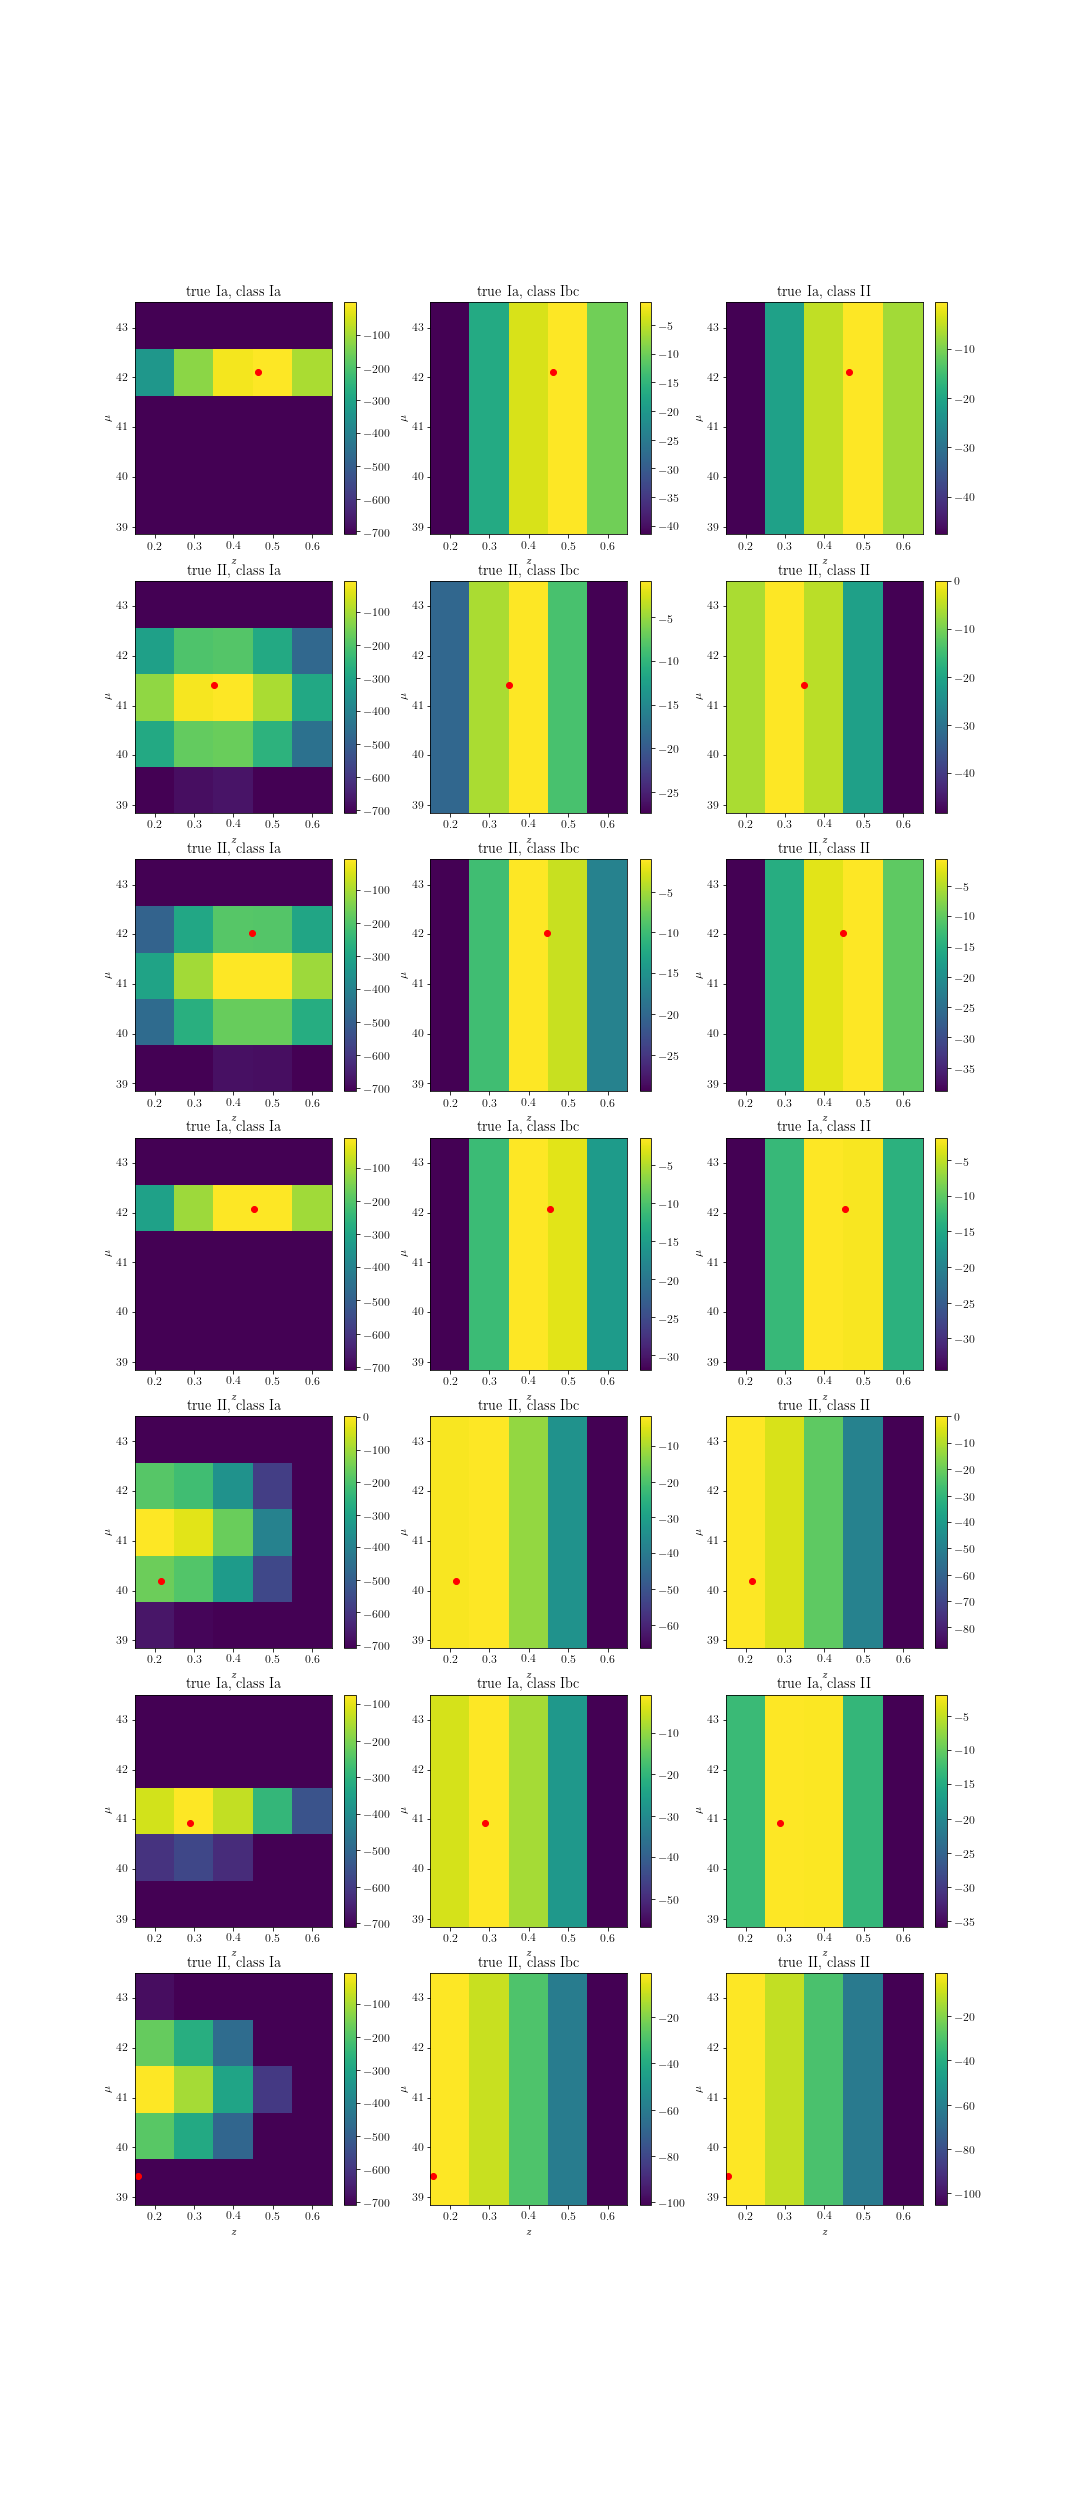
\includegraphics[width=0.5\textwidth]{fig/lc_likelihoods.png}
		\caption{SN posteriors.  
		(a few ``sheetcakes" of different true types)  \textbf{(@aimalz Add this plot.) 
		(Let's make this a 3x3 similar to the confusion matrix plot above.)}}
		\label{fig:SNposts}
	\end{center}
\end{figure}

\textbf{(Discuss potential ways to complicate this in a realistic way.)}

\subsubsection{Lightcurve fitting model}
\label{sec:snlcinterim}

An interim prior $p(t, z, \mu | \textul{\Phi}^{*})$ may be the supernova type-redshift-distance modulus distribution observed in a previous survey (training set) in the case of a template-based (machine learning) method for deriving interim posteriors.  
In our mock data, we choose an interim prior defined by hyperparameters $\textul{\Phi}^{*}$ that contains a perturbed version of the true redshift-dependent type proportion parameters $\textul{\phi}'$ representing an initial guess and anontrivial distribution in the space of distance modulus.  
We take a the distance modulus from Equation \ref{eq:distmod} evaluated at interim prior cosmological parameters $\vec{\Omega}^{*}$ from WMAP, including its error bars to produce a broad distribution in the space of distance modulus.

\newpage

\begin{figure}
	\begin{center}
		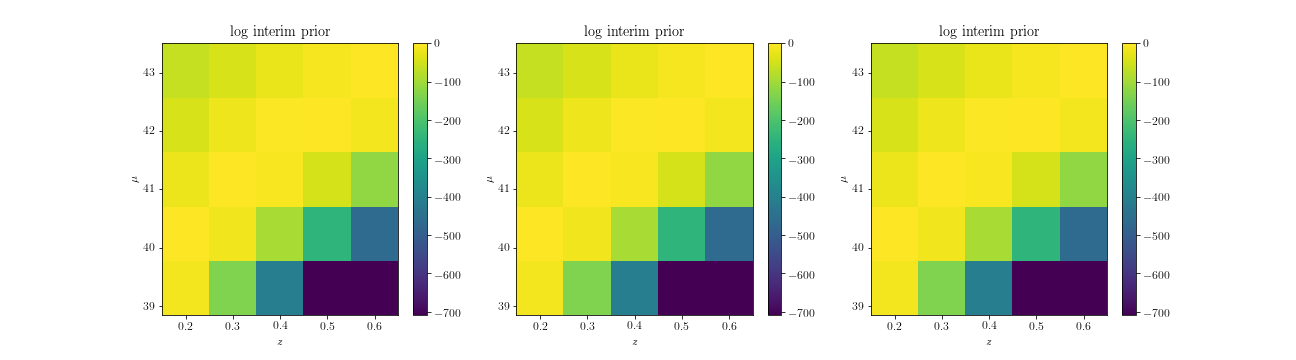
\includegraphics[width=0.5\textwidth]{fig/lc_interim.png}
		\caption{The SN interim prior.}
		\label{fig:SNintpr}
	\end{center}
\end{figure}

\newpage

\subsubsection{Supernova selection function}
\label{sec:snlcselection}

In order to estimate the observed selection function $p(\textul{\ell} | \vec{\alpha})$ which will dominate any supernova survey, we simulate two different surveys (in this case the LSST WFD survey and the Deep Drilling Field) and compute the ratio of the number of supernovae simulated in the survey to the number `detected' or recovered, and work in the space of type and redshift:

\begin{equation}
    \label{eq:snlcselfunwords}
    p(t, z | \vec{\alpha}) = \frac
    {\quad \left|\frac
    		{N_{\mathrm{SNe,recovered}}(t,z)}
    		{N_{\mathrm{SNe, simulated}}(t,z)}\right|_\mathrm{WFD}\quad}
    {\left|\frac
    	{N_{\mathrm{SNe, recovered}}(t,z)}
    	{N_{\mathrm{SNe, simulated}}(t,z)}\right|_\mathrm{DDF}}.
\end{equation}

%Though the selection function $p(\textul{\ell} | \vec{\alpha})$ for a survey occurs in the space of lightcurves $\textul{\ell}$, it is always projected into the space of lightcurve fit parameters. 
%In the equation above, we assume that is flat in $\mu$-space but non-trivial in type and redshift space. 


%the s We use a selection function that is flat with respect to the distance modulus but has nontrivial structure in the space of type and redshift.  Our empirical selection function is based on the ratio of the recovery rates of supernovae as a function of type and redshift in two simulated surveys, one representing a realistic observing strategy, LSST's wide-fast-deep (WFD) strategy, and one representing a best case observing strategy, LSST's deep drilling field (DDF) strategy,

\textbf{(@reneehlozek: Note that the selection function is NOT flat in mu space - we need to talk about this, since it will explicitly depend on the magnitude (that's how they are detected)} 

From this procedure, we obtain a normalized function evaluated over three supernova types and five discrete redshifts.

\begin{figure}
	\begin{center}
		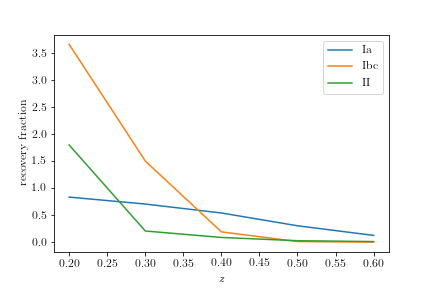
\includegraphics[width=0.5\textwidth]{fig/lc_sel_func.png}
		\caption{The SN selection function.  \textbf{(@reneehlozek This needs to be adjusted for survey volume.)}}
		\label{fig:SNselfun}
	\end{center}
\end{figure}

\subsection{Host galaxy photometry-based PDFs}
\label{sec:hostpdf}

Each host galaxy in the sample must have a one-dimensional probability distribution, which will be an interim posterior, over redshift, combined as
\begin{widetext}
\begin{align}
    \label{eq:fullhostpdf}
    p(z | \vec{f}_{i}, \vec{\beta}, \textul{\varphi}^{*}) = p(z | z_{i}', \vec{\beta}, \textul{\varphi}^{*}) &= p(z | z_{i}')\ p(z | \textul{\varphi}^{*}) p(z | \vec{\beta}),
\end{align}
or, in words
\begin{eqnarray}
    \label{eq:fullhostpdfwords}
    [\textrm{host galaxy post-selection interim posterior}]_{i} &=&[\textrm{photometric redshift posterior}]_{i}\nonumber \\ &\times&\ \textrm{redshift distribution interim prior}\ \times\ \textrm{host galaxy selection function} \nonumber \\.
\end{eqnarray}
\end{widetext}

Sections \ref{sec:hostposterior}, \ref{sec:hostinterim}, and \ref{sec:hostselection} cover the production of the photometric redshift posteriors, the redshift distribution interim prior, and host galaxy selection function respectively.

\subsubsection{Host galaxy photometry data model}
\label{sec:hostposterior}

We present our model for emulating one-dimensional posteriors $p(z | \vec{f}_{i})\equiv p(z | z_{i}')$.  
We use a nonparametric piecewise constant parametrization because it is flexible enough to accommodate many shapes for the redshift posterior.  
For simplicity, we choose a Gaussian distribution $\mathcal{N}(\hat{z}_{i}, \sigma_{f}^{2})$ with a variance $\sigma_{f}^{2}$ shared by the entire dataset and a mean of $\hat{z}_{i}\sim \mathcal{N}(z'_{i}, \sigma_{f}^{2})$ of the same variance with a mean of the true redshift $z'_{i}$, the true redshift.  
\textbf{(If we use more complex/realistic for photo-$z$ PDFs, we will need to use a more sophisticated data generation procedure, as in \texttt{chippr}.)}  
Examples of these photo-$z$ posteriors are shown in Fig. \ref{fig:pzs}.  
We reiterate that the piecewise constant parametrization does not force the host galaxy redshift posteriors to take this simplistic form.

\begin{figure}
	\begin{center}
		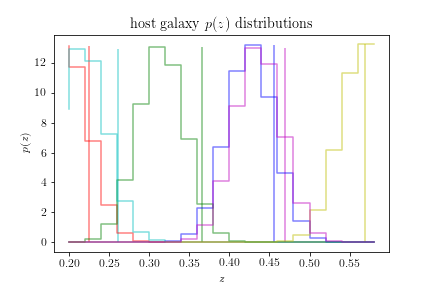
\includegraphics[width=0.5\textwidth]{fig/host_pzs.png}
		\caption{Examples of mock photo-$z$ posteriors.  \textbf{(@aimalz Actually replace this with that SDSS $n(z)$.)}}
		\label{fig:pzs}
	\end{center}
\end{figure}

\subsubsection{Host galaxy photo-$z$ fitting model}
\label{sec:hostinterim}

The interim prior $p(z | \vec{\varphi}^{*})$ is a normalized redshift distribution that is often a best guess for that of the survey in question, based on one from a previous survey or training set for a photometric redshift PDF code.  
Here, we use that of the Sloan Digital Sky Survey (SDSS) Data Release 7 (DR7) that covers the same redshift range as the redshift-dependent supernova type proportions.  \textbf{(@aimalz Do this ASAP!)}

\begin{figure}
	\begin{center}
		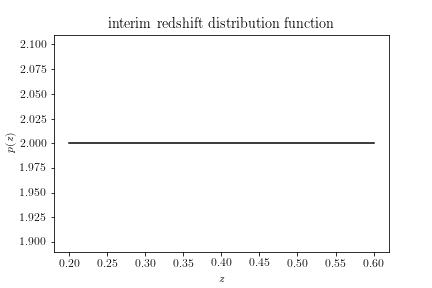
\includegraphics[width=0.5\textwidth]{fig/pz_interim_prior.png}
		\caption{The redshift distribution interim prior binned down to the resolution of the SN selection function. 
		The interim prior is normalised to integrate to unity within the redshift range. 
		(\textbf{This won't be flat once it is changed in the code to be the host galaxy photo-z selection function from SDSS DR7.})}
		\label{fig:hostintpr}
	\end{center}
\end{figure}

\subsubsection{Host galaxy selection function}
\label{sec:hostselection}

Though the host galaxy selection function $p(\vec{f} | \vec{\beta})$ is defined in the space of host galaxy photometry $\vec{f}$, it is projected into redshift space as $p(z | \vec{\beta})$.  \textbf{(@aimalz Do this to Buzzard data.)}  
The \texttt{Buzzard} simulation produces a catalog of galaxy redshifts, spectral energy distributions (SEDs), photometric magnitudes, and signal-to-noise rates.  
Knowing the magnitude limits and signal-to-noise cuts of LSST's WFD and DDF survey strategies, we can calculate the recovery fraction as a function of redshift and SED under each.  
(At this point, we could impose a prior on SED due to the known correlation between a galaxy's SED and the type of supernova likely to occur in it, although we do not include that complication in this study.)  
We integrate these fractions over SED and take the ratio as
\begin{equation}
    \label{eq:hostselfunwords}
     p(t, z | \vec{\beta}) = \frac
     {\quad\left|\frac
     	{N_{\mathrm{gal, recovered}}(t,z)}
     	{N_{\mathrm{gal,simulated}}(t,z)}\right|_\mathrm{WFD}\quad}
     {\left|\frac
     		{N_{\mathrm{gal, recovered}}(t,z)}
     		{N_{\mathrm{gal,simulated}}(t,z)}\right|_\mathrm{DDF}}
   % p(z | \vec{\beta}) = \frac{\frac{\mathrm{number\ of\ recovered\ galaxies\ at\ redshift\ }z\mathrm{\ in\ WFD}}{\mathrm{number\ of\ simulated\ galaxies\ at\ redshift\ }z\mathrm{\ in\ WFD}}}{\frac{\mathrm{number\ of\ recovered\ galaxies\ at\ redshift\ }z\mathrm{\ in\ DDF}}{\mathrm{number\ of\ simulated\ galaxies\ at\ redshift\ }z\mathrm{\ in\ DDF}}}
\end{equation}
to obtain $p(z | \vec{\beta})$.

\begin{figure}
	\begin{center}
		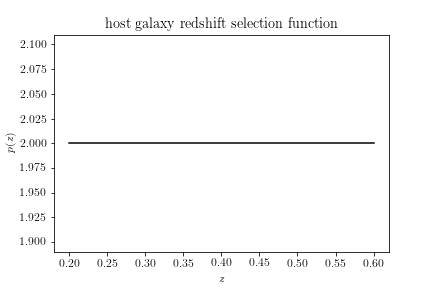
\includegraphics[width=0.5\textwidth]{fig/pz_sel_fun.png}
		\caption{The host galaxy selection function.}
		\label{fig:hostselfun}
	\end{center}
\end{figure}

\subsection{Mock data product}
\label{sec:finalmockdata}

Finally, we have all the components necessary\dots  \textbf{(@aimalz Paste in the equation with all these pieces and tie in to flowchart.)}

\begin{figure*}
	\begin{center}
		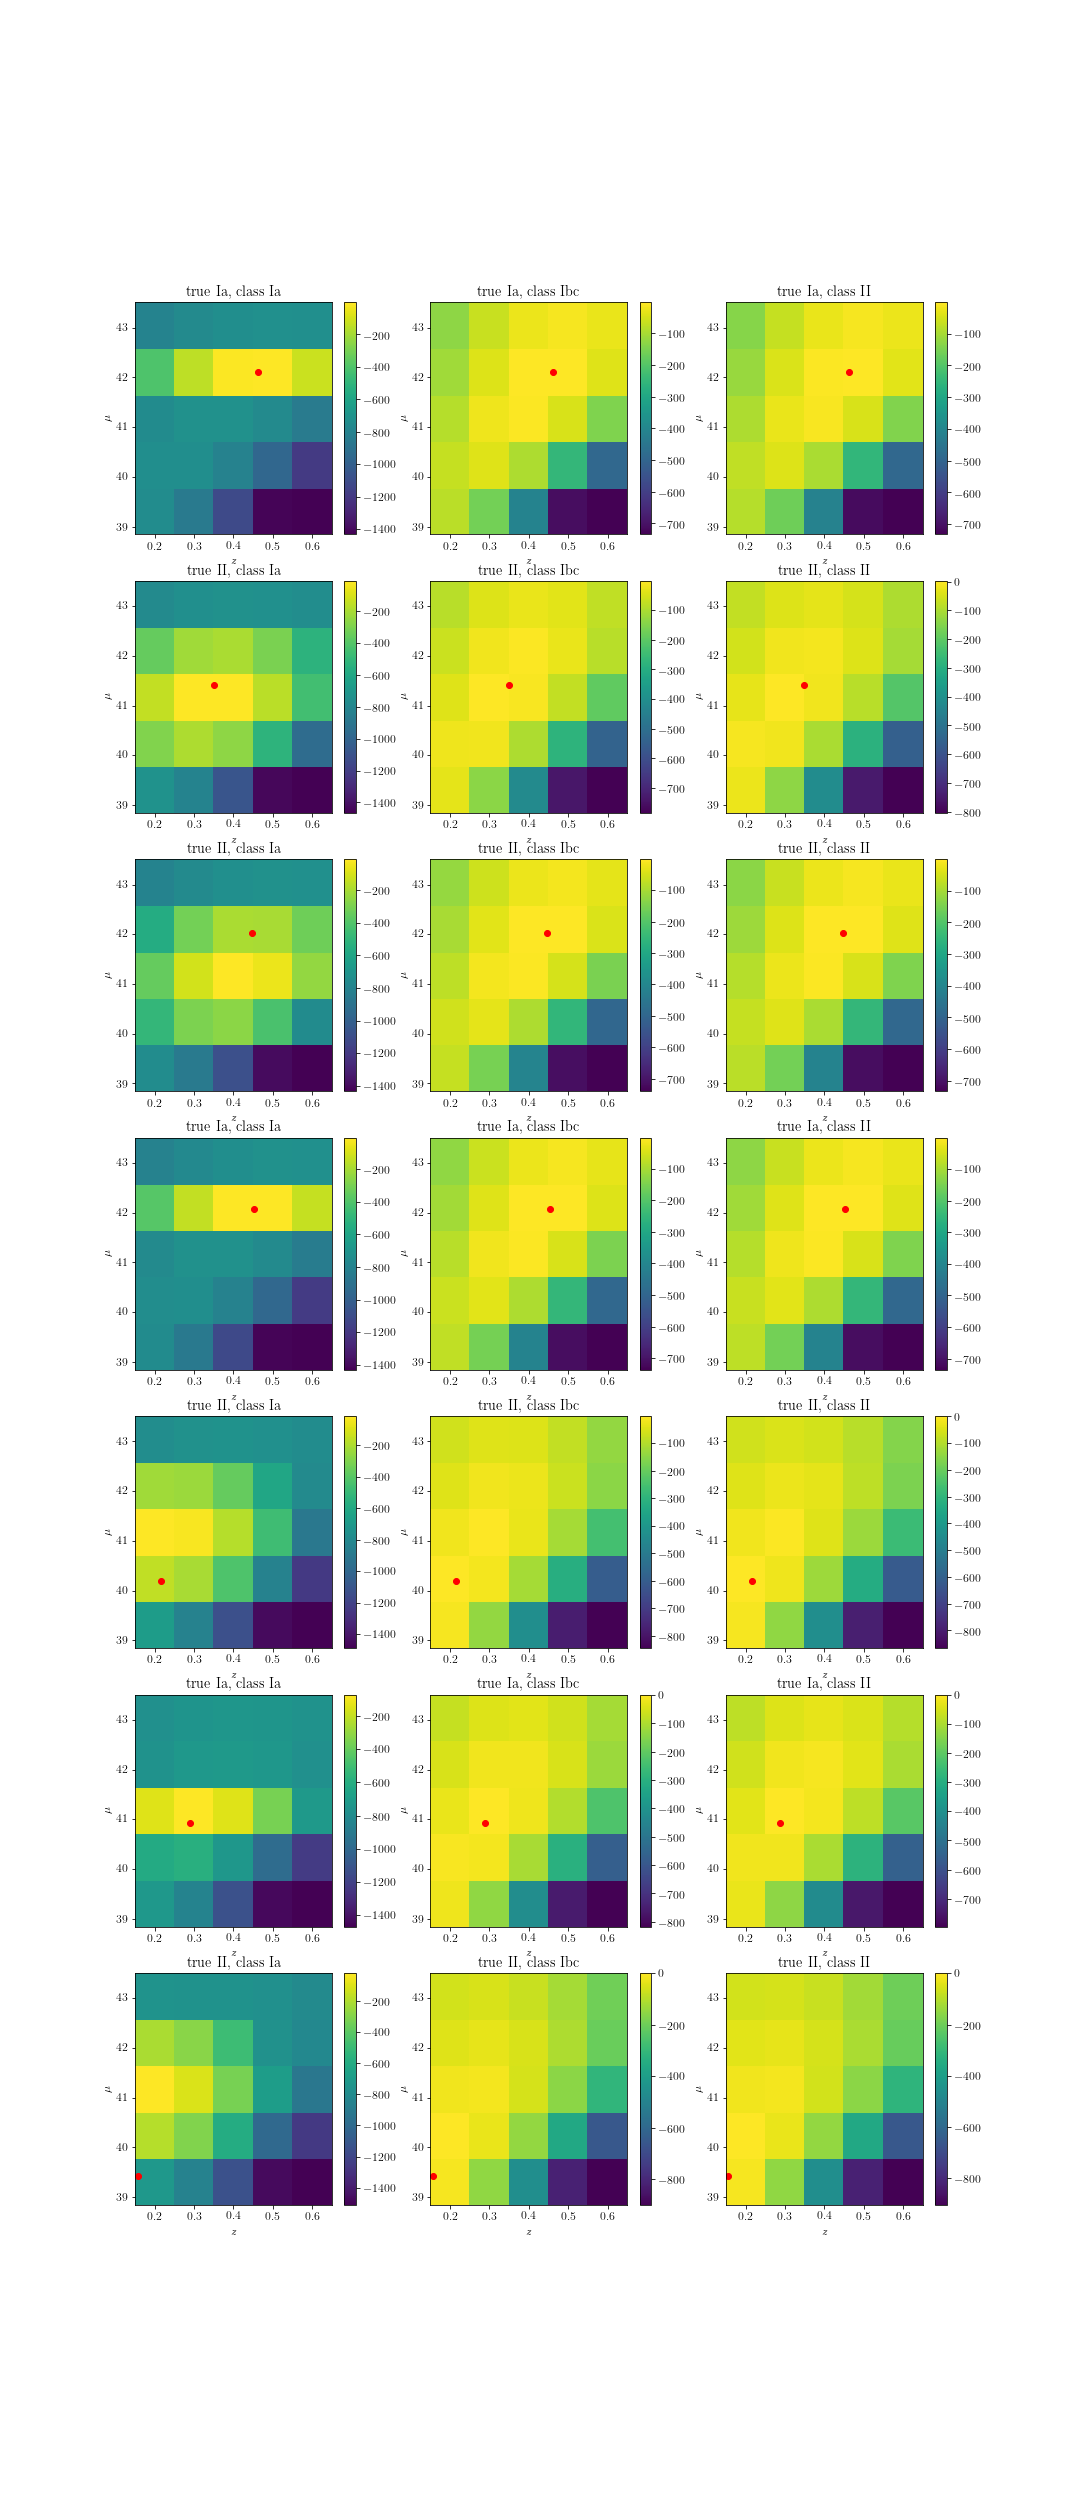
\includegraphics[width=0.5\textwidth]{fig/out_interim_posteriors.png}
		\caption{A depiction of ``the sheetcake" for a handful of supernovae.}
		\label{fig:indieposts}
	\end{center}
\end{figure*}

%\clearpage

\section{Results}
\label{sec:results}
Once we have set up the overall mock data structure, that are drawn from the joint interim posteriors, we can compare the performance of \scippr against different ways of handling photometric supernova data. 
In order to process the data in more traditional approaches, we will need to `project' the data on to a Hubble diagram. 
This is artificial in the case of \scippr, as it be construction avoids the 2-dimensional Hubble diagram entirely.

We make use of the {\tt emcee} \citep{emcee} sampler throughout and use the Gelman-Rubin convergence test, requiring $R > xxx$ for convergence.

\subsection{Comparison to `standard' approaches}
\label{sec:naive}
While the community is moving towards cosmology with photometric supernova sample \cite{Campbell_2013, hlozek_photometric_2012, Jones_2017}, the gold standard still remains using a spectroscopic subset of 'known' SNe Ia to perform cosmological inference. 
We will denote this subclass of data the \textit{spectro} subset, which will be analysed in the usual $\chi^2$ approach. 
For this data we will assume that given the SN spectrum, the redshift of the supernova is known to spectroscopic precison.

In addition, a cut on probability, and clipping of $5\sigma$-outliers can be used to ensure a sample as `clean' as possible \citep[eg. see][]{Campbell_2013}. 
We will also assume that the redshift of the host is known spectroscopically. 
We will denote this sample as the \textit{probcut} subset.

The performance of \scippr compared to the simpler inference methods on both the full data set, and on the subsets above is shown in Figure~\ref{fig:scippr_final1}.
%\begin{itemize}
 %   \item all data: plot mode version of hubble diagram with colors for type probabilities
  %  \item spec-like sample: redshift interim prior from spec survey, photo-z PDF both precise and accurate, cut in type probability, cut in mu spread/mode, make hubble diagram with colors for type probabilities, do cosmology
   % \item probability cut: probability cuts to choose point estimators for hubble diagram, plus outlier cut, plus most precise/accurate photo-z PDF (basically above but including probability of type), do cosmology
%\end{itemize}

\begin{figure}
	\begin{center}
	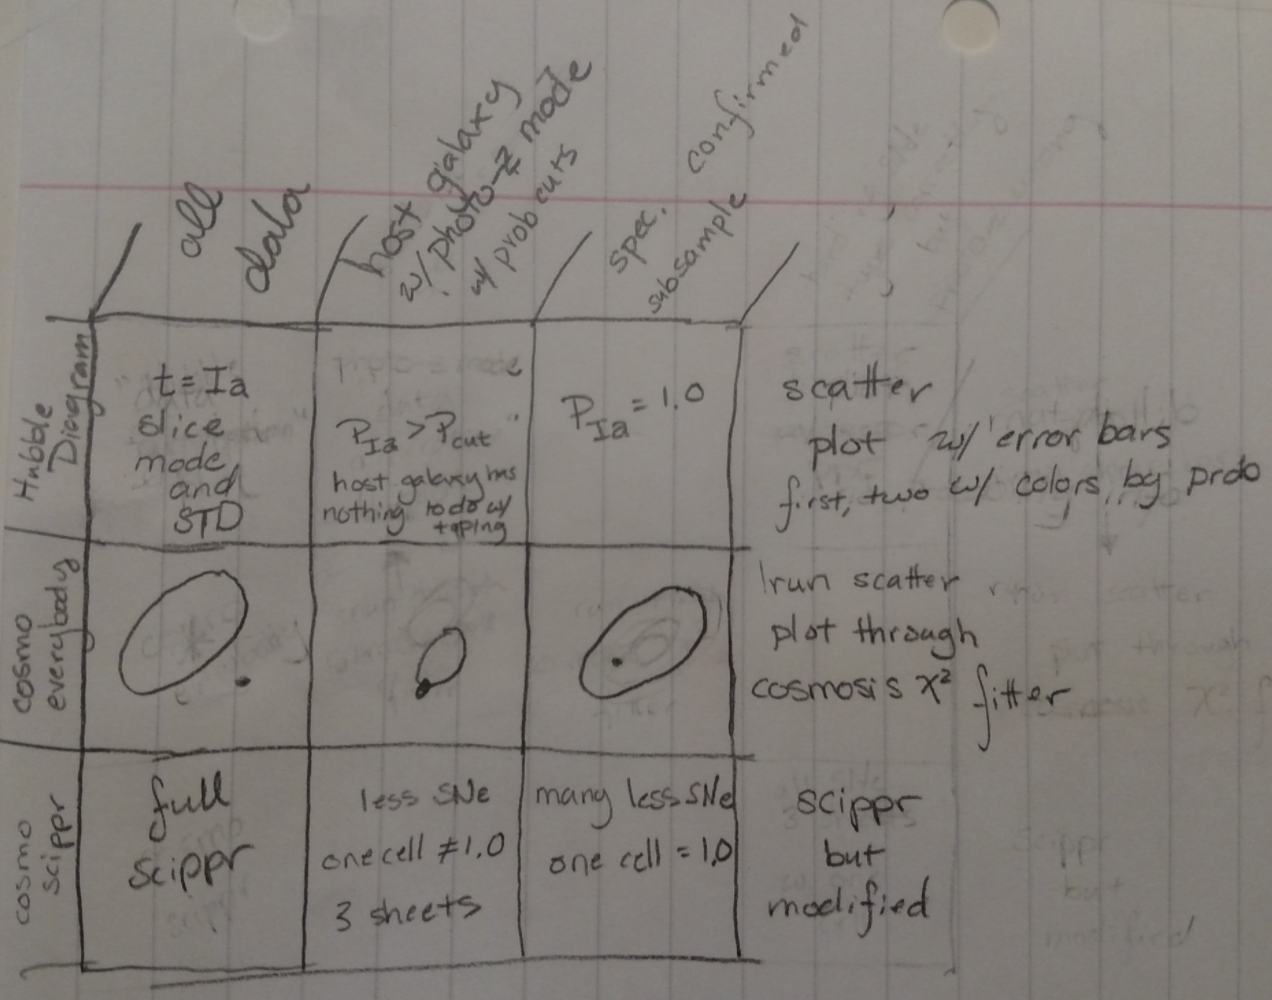
\includegraphics[width=0.5\textwidth]{fig/results1.png}

	\caption{Comparing the results for the full data set, a subset of the data based on probability cuts, and a subset of the data based on spectroscopic cuts.}
	\label{fig:results1}
	\end{center}
\end{figure}

\begin{figure}
	\begin{center}
	    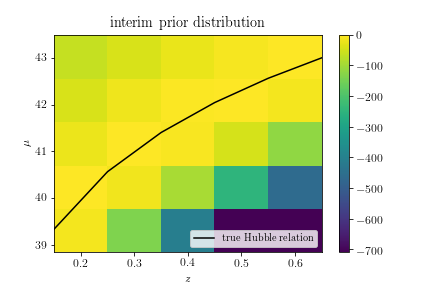
\includegraphics[width=0.3\textwidth]{fig/sn_interim_prior.png}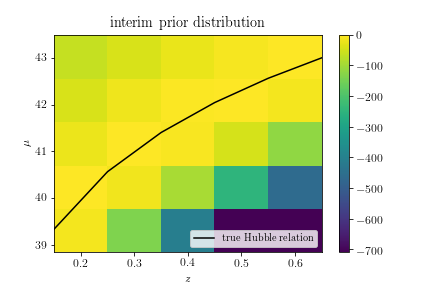
\includegraphics[width=0.3\textwidth]{fig/sn_interim_prior.png}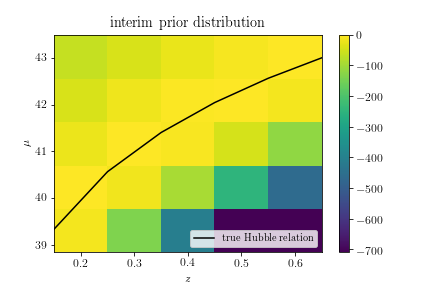
\includegraphics[width=0.3\textwidth]{fig/sn_interim_prior.png}\\
		\includegraphics[width=0.3\textwidth]{fig/final_constraints.png}\includegraphics[width=0.3\textwidth]{fig/final_constraints.png}\includegraphics[width=0.3\textwidth]{fig/final_constraints.png}\\
		\includegraphics[width=0.3\textwidth]{fig/final_constraints.png}\includegraphics[width=0.3\textwidth]{fig/final_constraints.png}\includegraphics[width=0.3\textwidth]{fig/final_constraints.png}
		\caption{The results of inference with SCIPPR using different cuts on the data.  
		Top row: Hubble diagram based on modes of PDFs.  
		Middle row: posterior inference of $w_{0}, w_{a}$ using $z, \mu$ values from Hubble diagram of modes of PDFs.  
		Bottom row: posterior inference of $w_{0}, w_{a}$ using the full PDFs.  
		Left column: the full dataset without cuts.  
		Middle column: spectroscopic-like cuts in redshift precision and type probability.  
		Right column: photometric-like cuts in type probability and using the mode of the photo-z PDF.}
		\label{fig:scippr_final1}
	\end{center}
\end{figure}


\subsection{Comparison to simpler photometric approaches}

While we expect \SCIPPR to perform well on spectroscopically-motivated methods, it is worth comparing the method to probabilistic approaches optimised for either photometric redshifts (like those used in the photo-$z$ community), or supernova probalities (like the \BEAMS methods, most recently updated with some attention to redshifts as zBEAMS \cite{Roberts_2017}).

To illustrate these sorts of scenarios, we will use \scippr, but restrict the inference in two different ways:

\begin{itemize}
    \item $p(z)$ \\
    Assume the full probabilistic $z, \mu$ information, but use only the SNIa `slice' of the \scippr ``sheetcake".
    \item `BEAMS'-like \\   
    Assume full probabilistic type but use the mode of the photo-$z$ PDF.
\end{itemize}

We compare the performance of \scippr restricted to the performance where we include all the relevant \scippr information in Figure~\ref{fig:scippr_final2}.

%\begin{itemize}
%    \item all data: scippr as is
%    \item naive probability:  keep probabilistic z, mu, stack Ia-only slices, do cosmology without hubble
%    \item BEAMS: keep probabilistic type, mode of photo-z PDF, do cosmology withiut hubble
%\end{itemize}


\begin{figure}
	\begin{center}
	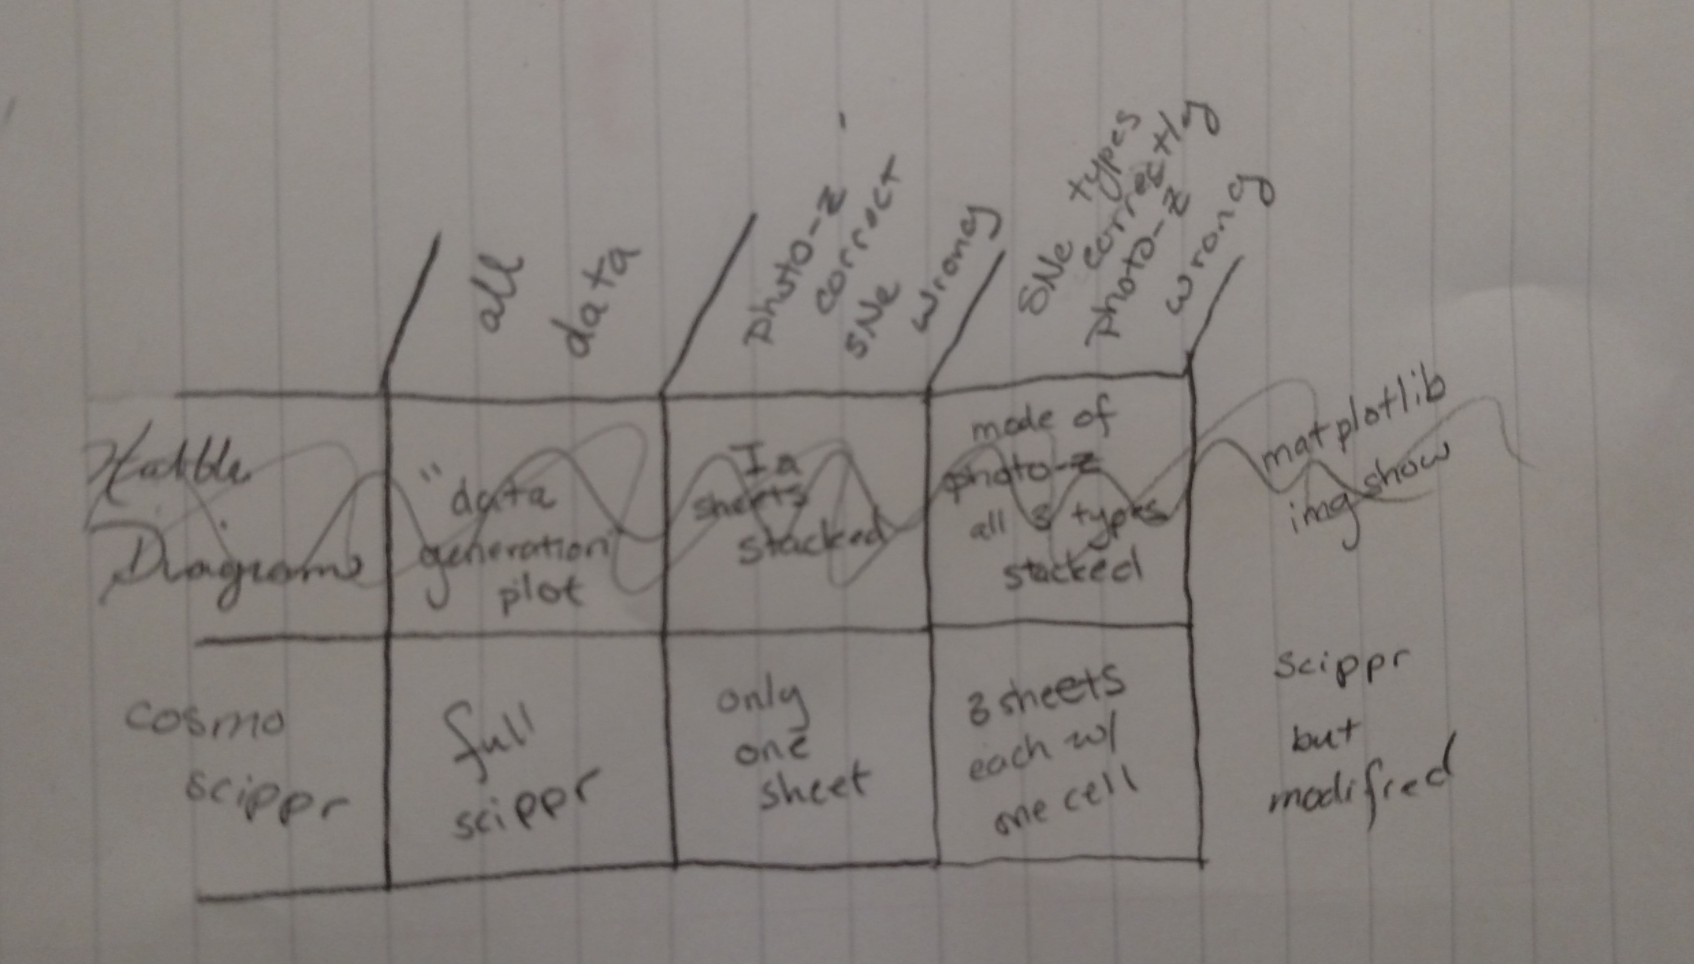
\includegraphics[width=0.5\textwidth]{fig/results2.png}
	\caption{Comparing the results for handling the full data set correctly, mishandling the supernovae types, and mishandling the photozs.}
	\label{fig:results2}
	\end{center}
\end{figure}

[contours in $w_0$, $w_a$ under scippr plus 3 choices in previous section]

\begin{figure}
	\begin{center}
		\includegraphics[width=0.3\textwidth]{fig/final_constraints.png}\includegraphics[width=0.3\textwidth]{fig/final_constraints.png}\includegraphics[width=0.3\textwidth]{fig/final_constraints.png}
		\caption{Posterior inference of $w_{0}, w_{a}$ under three methods for handling probabilistic data.  
		Left: SCIPPR approach.  Middle: stacking Ia information.  
		Right: BEAMS with mode of redshift and distance modulus distributions.}
		\label{fig:scippr_final2}
	\end{center}
\end{figure}

\section{Conclusion \& Future Directions}
\label{sec:conclusion}

%\acknowledgments

\clearpage

\bibliography{references}

\clearpage

\begin{appendix}
\label{appendix:derivation}

Starting with Equation~\ref{eq:independence}, we marginalize over the latent variables, showing how the unobservable variables enter the inference:
\begin{align}
\label{eq:marginalization}
p(\textul{\ell}_{n}, \vec{f}_{n} | \vec{\Omega}, \textul{\phi}) &= \iiint p(\textul{\ell}_{n}, \vec{f}_{n} | \mu_{n}, z_{n}, t_{n})\ p(\mu_{n}, z_{n}, t_{n} | \vec{\Omega}, \textul{\phi})\ d\mu_{n}\ dz_{n}\ dt_{n}
\end{align}
 
  We note that Eq. \ref{eq:marginalization} calls for the likelihoods $\{p(\textul{\ell}_{n}, \vec{f}_{n} | \mu_{n}, z_{n}, t_{n})\}_{N}$ containing the supernova lightcurve and host galaxy photometry \textit{given} some particular values of distance modulus, redshift, and type. 
  What we have at our disposal are the \textit{interim posteriors}  $\{p(\mu_{n}, z_{n}, t_{n} | \textul{\ell}_{n}, \vec{f}_{n}, \vec{\theta}, \textul{\xi}, \vec{\alpha}, \vec{\beta})\}_{N}$, which are probabilities of the distance modulus, redshift, and type given fixed values for the supernova lightcurve, host galaxy photometry, and priors from the data analysis procedure and survey program.

We thus must transform our expression Eq.~\ref{eq:marginalization} to be in terms of quantities at our disposal. 
This is achieved by multiplying the likelihood by an inspired factor of unity, in terms of the interim posteriors.
\begin{align}
\label{eq:unity}
p(\textul{\ell}_{n}, \vec{f}_{n} | \mu_{n}, z_{n}, t_{n}) &= p(\textul{\ell}_{n}, \vec{f}_{n} | \mu_{n}, z_{n}, t_{n})\ \frac{p(\mu_{n}, z_{n}, t_{n} | \textul{\ell}_{n}, \vec{f}_{n},\vec{\theta}, \textul{\xi}, \vec{\alpha}, \vec{\beta})}{p(\mu_{n}, z_{n}, t_{n} | \textul{\ell}_{n}, \vec{f}_{n}, \vec{\theta}, \textul{\xi}, \vec{\alpha}, \vec{\beta})}
\end{align}
We expand the denominator of the fraction on the right hand side according to Bayes' Rule: $p(\mu_{n}, z_{n}, t_{n} | \textul{\ell}_{n}, \vec{f}_{n}, \vec{\theta}, \textul{\xi}, \vec{\alpha}, \vec{\beta}) = p(\mu_{n}, z_{n}, t_{n} | \vec{\theta}, \textul{\xi}, \vec{\alpha}, \vec{\beta})\ p(\textul{\ell}_{n}, \vec{f}_{n} | \mu_{n}, z_{n}, t_{n}, \vec{\theta}, \textul{\xi}, \vec{\alpha}, \vec{\beta})$ to obtain (\textbf{RH: we don't describe how a term was added to the numerator here})

\begin{align}
\label{eq:expand}
p(\textul{\ell}_{n}, \vec{f}_{n} | \mu_{n}, z_{n}, t_{n}) &= p(\textul{\ell}_{n}, \vec{f}_{n} | \mu_{n}, z_{n}, t_{n})\ p(\mu_{n}, z_{n}, t_{n} | \textul{\ell}_{n}, \vec{f}_{n},\vec{\theta}, \textul{\xi}, \vec{\alpha}, \vec{\beta})\ \frac{p(\textul{\ell}_{n}, \vec{f}_{n} | \vec{\theta}, \textul{\xi}, \vec{\alpha}, \vec{\beta})}{p(\mu_{n}, z_{n}, t_{n} | \vec{\theta}, \textul{\xi}, \vec{\alpha}, \vec{\beta})\ p(\textul{\ell}_{n}, \vec{f}_{n} | \mu_{n}, z_{n}, t_{n}, \vec{\theta}, \textul{\xi}, \vec{\alpha}, \vec{\beta})}
\end{align}
The most daunting term in the denominator of the above can be simplified using the independence of hierarchical models as:
\begin{align}
\label{eq:breakdown}
p(\textul{\ell}_{n}, \vec{f}_{n} | \mu_{n}, z_{n}, t_{n}, \vec{\theta}, \textul{\xi}, \vec{\alpha}, \vec{\beta}) &= p(\textul{\ell}_{n}, \vec{f}_{n} | \mu_{n}, z_{n}, t_{n})\ p(\textul{\ell}_{n}, \vec{f}_{n} | \vec{\theta}, \textul{\xi}, \vec{\alpha}, \vec{\beta}).
\end{align}
Noting the presence of $p(\textul{\ell}_{n}, \vec{f}_{n} | \mu_{n}, z_{n}, t_{n})$ and $p(\textul{\ell}_{n}, \vec{f}_{n} | \vec{\theta}, \textul{\xi}, \vec{\alpha}, \vec{\beta})$ in both the numerator and denominator for $p(\textul{\ell}_{n}, \vec{f}_{n} | \mu_{n}, z_{n}, t_{n})$, we cancel the like terms to express the individual likelihoods in terms of known quantities, obtaining
\begin{align}
\label{eq:cancellation}
p(\textul{\ell}_{n}, \vec{f}_{n} | \mu_{n}, z_{n}, t_{n}) &= \frac{p(\mu_{n}, z_{n}, t_{n} | \textul{\ell}_{n}, \vec{f}_{n}, \vec{\theta}, \textul{\xi}, \vec{\alpha}, \vec{\beta})}{p(\mu_{n}, z_{n}, t_{n} | \vec{\theta}, \textul{\xi}, \vec{\alpha}, \vec{\beta})}.
\end{align}
We are now ready to plug the individual likelihoods into Eq. \ref{eq:marginalization}, leading to
\begin{align}
\label{eq:buildup}
p(\textul{\ell}_{n}, \vec{f}_{n} | \vec{\theta}, \textul{\phi}) &= \iiint p(\mu_{n}, z_{n}, t_{n} | \textul{\ell}_{n}, \vec{f}_{n}, \vec{\theta}^{*}, \textul{\phi}^{*})\ \frac{p(\mu_{n}, z_{n}, t_{n} | \vec{\theta}, \textul{\phi})}{p(\mu_{n}, z_{n}, t_{n} | \vec{\theta}^{*}, \textul{\phi}^{*})}\ d\mu_{n}\ dz_{n}\ dt_{n}
\end{align}
Finally, we plug Eq. \ref{eq:buildup} back into Eq. \ref{eq:independence}.
\begin{align}
\label{eq:plugin}
p(\{\textul{\ell}_{n}, \vec{f}_{n}\}_{N} | \vec{\Omega}, \textul{\phi}) &= \prod_{n}^{N}\ \iiint p(\mu_{n}, z_{n}, t_{n} | \textul{\ell}_{n}, \vec{f}_{n}, \vec{\theta}, \textul{\xi}, \vec{\alpha}, \vec{\beta})\ \frac{p(\mu_{n}, z_{n}, t_{n} | \vec{\Omega}, \textul{\phi})}{p(\mu_{n}, z_{n}, t_{n} | \vec{\theta}, \textul{\xi}, \vec{\alpha}, \vec{\beta})}\ d\mu_{n}\ dz_{n}\ dt_{n}
\end{align}
And finally, we plug the product back into Eq. \ref{eq:bayes} to obtain
\begin{align}
\label{eq:wrapup}
p(\vec{\Omega}, \textul{\phi} | \{\textul{\ell}_{n}, \vec{f}_{n}\}_{N}) &\propto p(\vec{\Omega}, \textul{\phi})\ \prod_{n}^{N}\ \iiint p(\mu_{n}, z_{n}, t_{n} | \textul{\ell}_{n}, \vec{f}_{n}, \vec{\theta}, \textul{\xi}, \vec{\alpha}, \vec{\beta})\ \frac{p(\mu_{n}, z_{n}, t_{n} | \vec{\Omega}, \textul{\phi})}{p(\mu_{n}, z_{n}, t_{n} | \vec{\theta}, \textul{\xi}, \vec{\alpha}, \vec{\beta})}\ d\mu_{n}\ dz_{n}\ dt_{n},
\end{align}
the posterior on cosmological parameters and redshift-dependent type proportions that we wish to sample, which is given as Eq.~\ref{eq:wrapupmain} in the main body of the paper.



It is very important to document the assumptions we make with this model:
\begin{enumerate}
	\item\label{it:completeness} The expression of Eq. \ref{eq:wrapupmain} is only as correct as the probabilistic graphical model of Fig. \ref{fig:pgm} is complete.
	\item\label{it:prior} We choose a prior probability distribution $p(\vec{\Omega}, \textul{\phi})$.
	\item\label{it:interimpriors} The interim prior parameters $\vec{\theta}$ and $\textul{\xi}$ are known and shared among all supernovae and host galaxies $n$.
	\item\label{it:selectionfunctions} The selection function parameters $\vec{\beta}$ and $\textul{\alpha}$ are known and shared among all supernovae and host galaxies $n$.
	\item\label{it:independence} All latent and observed parameters associated with the supernovae and their host galaxies are statistically independent from the latent and observed parameters of all other supernovae and their host galaxies.
	\item\label{it:accuracy} The interim posterior distributions $\{p(z_{n} | \vec{f}_{n}, \vec{\theta}, \vec{\beta})\}_{N}$ and $\{p(t_{n}, z_{n}, \mu_{n} | \textul{\ell}_{n}, \textul{\xi}, \vec{\alpha})\}_{N}$ are accurate.
\end{enumerate}
There are a few caveats to these assumptions.  

Item \ref{it:completeness} is present with any approach. In order to make the problem tractable, we need to make some simplifying assumptions. 
The hierarchical Bayesian model provides the easiest framework for extending the model in different ways. 

% , as no model can include every aspect of the physics -- to make any problem tractable, we must make simplifications.  The hierarchical Bayesian approach, however, easily accommodates complications so is extensible to more refined models.

As in all analyses, care must be taken when choosing a prior distribution, as it can impart a bias on the resulting inference, but it can be an advantage when the data quality is poor and there are already trustworthy constraints on the parameters in question.  
We will nonetheless try to minimize the information imparted to the posterior by the prior.


% Skeptics of Bayesian statistics often cite item \ref{it:prior} as a major weakness of this approach.  It is true that choosing a prior distribution can 

It is noted that this model may be adapted to the cases when Items \ref{it:interimpriors} and \ref{it:selectionfunctions} are violated, which will be the case if the interim posteriors are not derived by a single method or if the photometry comes from a combination of surveys.  

Item \ref{it:independence} is never truly valid in that all data observed by a single instrument are correlated, for example, but if the data primarily inform us about the phenomenon in question and we believe the principle of the universality of physics, it is a safe assumption; furthermore, virtually no statistical analysis would be possible without it, so all alternative methods already make this assumption.

It may seem to go without saying, but Item \ref{it:accuracy} can be difficult to guarantee.  
As will be discussed further in Sec. \ref{sec:data}, there is as yet no established method for producing the interim posterior distributions, and validating any such method's accuracy will be a challenge, as it has proven to be for photo-$z$ PDFs.

\section{Supernova rates}
We discuss the specific supernova rate computations here.


\subsubsection{Supernova Type II Rate with Redshift}
\label{sec:TypeIIRate}

To determine the rate of SNII per unit comoving volume we will basically apply the approach by Forster et al. 2006/Strogler et al. 2004 adapted to SNe II following Botticella et al. 2012.

The rate of SNe II per unit time per unit comoving volume ($R_{II}$) is given by the star formation rate ($SFR$) per unit time per unit comoving volume convolved with the number of stars crearted that will explode as SNe II.

\begin{align}
	\label{eq:rateII_1}
	R_{II} = K_{II} \times SFR
\end{align}

First, we must calculate the fraction of stars that explode as SN II:

\begin{align}
\label{eq:rateII_2}
K_{II} = \frac{\int_{m_{l,II}}^{m_{u,II}} \phi(m) \mathrm{d}m}{\int_{m_{l}}^{m_{u}} m\phi(m) \mathrm{d}m}
\end{align}

When we integrate from a minimum mass, $m_{l,II}$, of 8 to a maximum mass, $m_{u,II}$, to 25 and assuming a Salpeter et al. (1955) IMF we get a rate of $6.027 \time 10^{-3}$.

We will use three different models of how the SFR evolutions with redshift: Cole et al. (2001), Horiuchi et al. (2011), and Madau et al. (2014)

\begin{figure}
	\begin{center}
		\includegraphics[width=0.5\textwidth]{fig/SNII_SFR.png}
		\caption{SFR evolutions with redshift: Cole et al. (2001), Horiuchi et al. (2011), and Madau et al. (2014).}
		\label{fig:SNII_SFR}
	\end{center}
\end{figure}

Next we will take the spectral model of Dessart et al. (2013) which is anchored to SN II 1999em, as a reference. 
We simulate its $r$-band light curve at different redshifts and convolve it with the LSST filters to see when it falls below the detection limit.

\begin{figure}
	\begin{center}
		\includegraphics[width=0.5\textwidth]{fig/spectral_model_SNII.png}
		\caption{SN II spectral model of Dessart et al. (2013): $M_{99em}=-16.6$; $M_{05J}=-17.2$}
		\label{fig:SNII_lc}
	\end{center}
\end{figure}

\begin{figure}
	\begin{center}
		\includegraphics[width=0.5\textwidth]{fig/SNII_lc_withz.png}
		\caption{The $r$-band lightcurve of spectral model of SN II 1999em shifted to a range of redshifts. 
		The horizontal dashed line indicates the limiting magnitude of LSST in the $r$-band in a single visit.}
		\label{fig:SNII_lc_withz}
	\end{center}
\end{figure}

For this model SN II, we compare the magnitude as a function of time and redshift, $m(t,z)$, with the limiting magnitude, $m_{lim}$, of the LSST camera to obtain the probability of detecting (the peak of) a SN at a given redshift, $\Delta_{t}(z)$. 
Then we estimate the number of detected SNe II per unit of redshift, $dN/dz$, using Equations 2 and 5 of Forster et al. (2006).

\begin{figure}
	\begin{center}
		\includegraphics[width=0.5\textwidth]{fig/number_SNII.png}
		\caption{The number of SN II detected, for each of the SFR models, as a function of redshift. 
		The total number of SN II for Horiuchi et al. 16985, Cole et al. 29207, and Madau et al.  18322. }
		\label{fig:SNII_lc_sfr}
	\end{center}
\end{figure}

Finally, we use a a sample of 10,000 SNe, simulated using MCMC on real parameters of CSP SNe II. 
We put each at 100 random redshifts from 0.01 to 1.20, so we have 1,000,000 SNe. 
Next we consider the magnitude at the end of the plateau phase, instead of the peak magnitude. 
This is because in SN II cosmology, we do not standardize the magnitude at peak, but either the magnitude at around the center of the plateau (for spectroscopic methods), or the length/brightness-decline of the plateau (for photometric methods).

We use the apparent magnitudes at the end of the plateau phase and k-correct the magnitudes. 
Then we measure $\Delta_t(z)$, selecting different magnitude limit depending on the filter we use for observations. 
Finally, we compare the number of supernovae as a function of redshift for the three different SFR models.

\begin{figure}
	\begin{center}
		\includegraphics[width=0.5\textwidth]{fig/number_SNII_withmagntiudescatter.png}
		\caption{The number of SN II detected, for each of the SFR models, as a function of redshift. 
		The total number of SN II for Horiuchi et al. 16985, Cole et al. 29207, and Madau et al.  18322. }
		\label{fig:SNII_lc_wz}
	\end{center}
\end{figure}

\begin{figure}
	\begin{center}
		\includegraphics[width=0.5\textwidth]{fig/relative_supernova_rate.png}
		\caption{The relative supernova rates as a function of redshift. 
		Sums to one at every redshift (but should actually integrate to one over type and redshift!).  \textbf{(@aimalz Also plot the "observed" version of this for our sample)}}
		\label{fig:relative_supernova_rates}
	\end{center}
\end{figure}


\subsubsection{Supernova Type Ia Rate with Redshift}
\label{sec:TypeIaRate}

To calculate the SNe Ia rate, one follows a very similar procedure to the one described above for the SN II objects, but now use the \cite{Hsiao2007} template to `observe' the SN with LSST, which we quantify by requiring that the object is detected at $5\sigma$ in a co-added difference image.

\subsubsection{Supernova Type Ibc Rate with Redshift}
\label{sec:TypeIbcRate}

\end{appendix}
%\end{strip}


% \begin{strip}
% \begin{appendix}
% \label{appendix:realism}
% \textbf{(@tinapeters put Section 3.1 here.)}
% \end{appendix}
% \end{strip}

\end{document}